\changeHierarchyStyle{breakable,before=\par\smallskip\centering,after=\par}

\newcommand{\cbase}[1][{}]{\V{c}_{s#1}}
\newcommand{\cbody}[1][{}]{\V{c}_{d#1}}
\newcommand{\cbasestate}[1][{}]{\hatV{c}_{s#1}}
\newcommand{\cbodystate}[1][{}]{\hatV{c}_{d#1}}

\newcommand{\cvbase}[1][{}]{\dotV{c}_{s#1}}
\newcommand{\cabase}[1][{}]{\ddotV{c}_{s#1}}
\newcommand{\cjbase}[1][{}]{\dddotV{c}_{s#1}}

\newcommand{\cvbody}[1][{}]{\dotV{c}_{d#1}}
\newcommand{\cabody}[1][{}]{\ddotV{c}_{d#1}}
\newcommand{\cjbody}[1][{}]{\dddotV{c}_{d#1}}

\newcommand{\cBase}{\V{C}_s}
\newcommand{\cvBase}{\dotV{C}_s}

\newcommand{\cop}[1][{}]{\V[#1]{p}}
\newcommand{\cstate}{\hatV{c}}
\newcommand{\cjerk}{\dddotV{c}}
\newcommand{\cJerk}{\dddotV{C}}
\newcommand{\cState}{\hatV{C}}


\chapter{MPC controller for Pepper}

This module implements \acs{MPC} problem for Pepper locomotion and balancing as
proposed in \cite{Lafaye2014humanoids} with minor variations.


%%%%%%%%%%%%%%%%%%%%%%%%%%%%%%%%%%%%%%%%%%%%%%%%%%%%%%%%%%%%%%%%%%%%%%%%%%%%%%%%%%%%%%%%%%%%%%%%%%%%%%
%%%%%%%%%%%%%%%%%%%%%%%%%%%%%%%%%%%%%%%%%%%%%%%%%%%%%%%%%%%%%%%%%%%%%%%%%%%%%%%%%%%%%%%%%%%%%%%%%%%%%%
%%%%%%%%%%%%%%%%%%%%%%%%%%%%%%%%%%%%%%%%%%%%%%%%%%%%%%%%%%%%%%%%%%%%%%%%%%%%%%%%%%%%%%%%%%%%%%%%%%%%%%
\section{Notation}

\begin{description}
    \item[$\cbase$] -- CoM position of the base;
    \item[$\cbody$] -- CoM position of the upper body;
    \item[$\cop$] -- position of the CoP.
    \item[$\cstate^x$] = $({c}^x_s, \dot{c}^x_s, \ddot{c}^x_s, {c}^x_d, \dot{c}^x_d, \ddot{c}^x_d)$;
    \item[$\cstate^y$] = $({c}^y_s, \dot{c}^y_s, \ddot{c}^y_s, {c}^y_d, \dot{c}^y_d, \ddot{c}^y_d)$;
    \item[$\cstate$] = $(\cstate^x, \cstate^y)$;
    \item[$T_k$] -- sampling interval;
    \item[$m_s$] -- mass of the base;
    \item[$m_d$] -- mass of the body;
    \item[$r_s$] -- radius of the base support;
\end{description}



%%%%%%%%%%%%%%%%%%%%%%%%%%%%%%%%%%%%%%%%%%%%%%%%%%%%%%%%%%%%%%%%%%%%%%%%%%%%%%%%%%%%%%%%%%%%%%%%%%%%%%
%%%%%%%%%%%%%%%%%%%%%%%%%%%%%%%%%%%%%%%%%%%%%%%%%%%%%%%%%%%%%%%%%%%%%%%%%%%%%%%%%%%%%%%%%%%%%%%%%%%%%%
%%%%%%%%%%%%%%%%%%%%%%%%%%%%%%%%%%%%%%%%%%%%%%%%%%%%%%%%%%%%%%%%%%%%%%%%%%%%%%%%%%%%%%%%%%%%%%%%%%%%%%
\section{Support area}

\begin{figure}[!ht]
    \centering{
        \pgfplotsset{
            every axis post/.style={
                scale=1,
                every x tick label/.style={font=\scriptsize}, % reduce font
                every y tick label/.style={font=\scriptsize}, % reduce font
                label style={font=\scriptsize},               % reduce font
            }
        }
        % This file was created by matlab2tikz.
%
%The latest updates can be retrieved from
%  http://www.mathworks.com/matlabcentral/fileexchange/22022-matlab2tikz-matlab2tikz
%where you can also make suggestions and rate matlab2tikz.
%
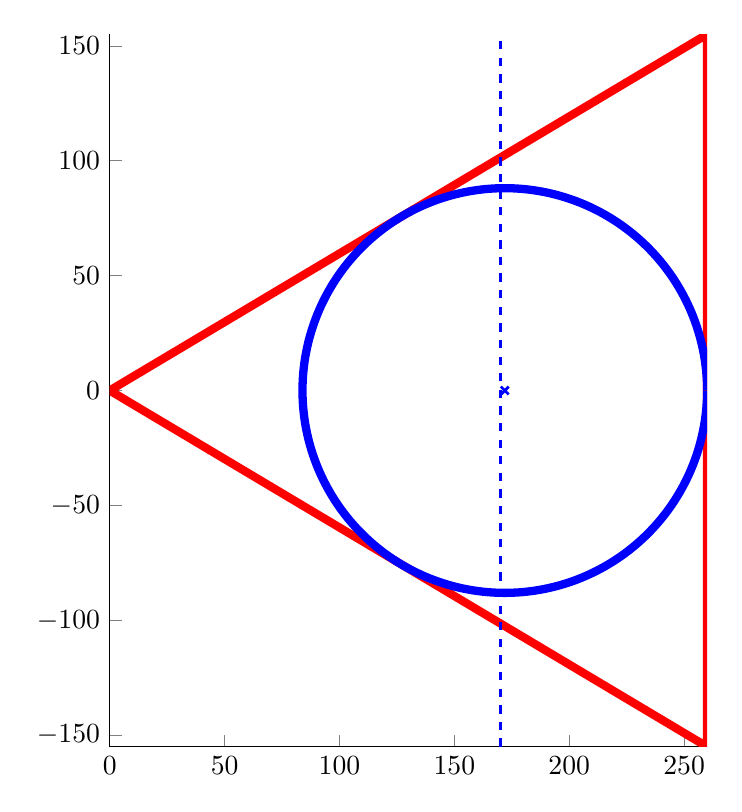
\begin{tikzpicture}

\begin{axis}[%
width=2.987in,
height=3.562in,
at={(1.522in,0.481in)},
scale only axis,
xmin=0,
xmax=260,
ymin=-155,
ymax=155,
axis background/.style={fill=white},
axis x line*=bottom,
axis y line*=left
]
\addplot [color=red,solid,line width=3.0pt,forget plot]
  table[row sep=crcr]{%
260	-155\\
260	155\\
0	0\\
260	-155\\
};
\addplot [color=blue,solid,line width=3.0pt,forget plot]
  table[row sep=crcr]{%
260	0\\
259.995597553285	0.880482005504181\\
259.982390653382	1.76087596354154\\
259.96038062097	2.64109383544994\\
259.929569657034	3.5210476001757\\
259.889960842643	4.40064926307564\\
259.841558138648	5.27981086471647\\
259.784366385277	6.15844448967065\\
259.718391301659	7.03646227530789\\
259.643639485247	7.91377642058129\\
259.56011841116	8.79029919480743\\
259.467836431436	9.66594294643931\\
259.366802774196	10.5406201118315\\
259.257027542722	11.4142432239963\\
259.138521714445	12.2867249213505\\
259.011297139849	13.1579779564515\\
258.875366541286	14.0279152047218\\
258.730743511703	14.8964496731616\\
258.577442513281	15.7634945090476\\
258.415478875994	16.628963008619\\
258.244868796069	17.4927686257469\\
258.065629334373	18.3548249805896\\
257.877778414702	19.2150458682298\\
257.681334821991	20.0733452672956\\
257.476318200437	20.9296373485625\\
257.262749051531	21.7838364835358\\
257.040648732009	22.6358572530139\\
256.810039451719	23.4856144556298\\
256.570944271396	24.3330231163715\\
256.323387100358	25.1779984950789\\
256.067392694118	26.0204560949185\\
255.802986651902	26.8603116708322\\
255.530195414094	27.6974812379624\\
255.24904625959	28.5318810800499\\
254.959567303073	29.3634277578059\\
254.661787492195	30.1920381172555\\
254.35573660469	31.0176292980534\\
254.041445245392	31.8401187417694\\
253.718944843174	32.6594242001446\\
253.388267647809	33.4754637433158\\
253.04944672674	34.2881557680089\\
252.702515961777	35.0974190056985\\
252.347510045707	35.9031725307353\\
251.984464478827	36.7053357684382\\
251.613415565389	37.503828503152\\
251.234400409977	38.2985708862685\\
250.84745691379	39.0894834442118\\
250.452623770856	39.8764870863852\\
250.049940464159	40.6595031130801\\
249.639447261694	41.4384532233466\\
249.22118521244	42.2132595228227\\
248.795196142254	42.9838445315241\\
248.361522649686	43.7501311915921\\
247.920208101726	44.5120428749992\\
247.47129662946	45.2695033912121\\
247.014833123661	46.0224369948104\\
246.550863230299	46.770768393061\\
246.079433345978	47.5144227534479\\
245.600590613292	48.2533257111546\\
245.114382916116	48.9874033765012\\
244.620858874815	49.7165823423329\\
244.120067841381	50.4407896913606\\
243.6120598945	51.1599530034531\\
243.096885834544	51.8740003628784\\
242.574597178489	52.5828603654955\\
242.045246154767	53.2864621258951\\
241.508885698037	53.9847352844873\\
240.965569443899	54.6776100145381\\
240.415351723525	55.3650170291521\\
239.858287558229	56.0468875882004\\
239.294432653963	56.7231535051956\\
238.723843395748	57.3937471541093\\
238.146576842035	58.0586014761356\\
237.562690718996	58.7176499863964\\
236.972243414759	59.3708267805896\\
236.375293973561	60.0180665415804\\
235.771902089849	60.6593045459318\\
235.162128102309	61.294476670378\\
234.546032987832	61.9235193982356\\
233.923678355415	62.5463698257562\\
233.295126440002	63.162965668416\\
232.660440096263	63.7732452671446\\
232.019682792302	64.3771475944907\\
231.372918603315	64.9746122607248\\
230.720212205183	65.5655795198781\\
230.061628868001	66.1499902757173\\
229.397234449555	66.7277860876537\\
228.727095388732	67.2989091765876\\
228.051278698881	67.8633024306861\\
227.369851961106	68.4209094110941\\
226.682883317515	68.9716743575782\\
225.990441464398	69.5155421941028\\
225.292595645364	70.0524585343374\\
224.589415644414	70.5823696870954\\
223.880971778961	71.1052226617031\\
223.167334892802	71.6209651732988\\
222.448576349031	72.1295456480612\\
221.724768022903	72.6309132283665\\
220.995982294647	73.1250177778745\\
220.262292042229	73.611809886542\\
219.523770634063	74.0912408755638\\
218.780491921675	74.5632628022406\\
218.032530232315	75.027828464773\\
217.27996036153	75.4848914069819\\
216.52285756568	75.934405922954\\
215.761297554413	76.3763270616122\\
214.995356483096	76.810610631211\\
214.225110945198	77.2372132037554\\
213.45063796463	77.6560921193434\\
212.672014988046	78.0672054904328\\
211.889319877093	78.4705122060288\\
211.102630900632	78.8659719357962\\
210.312026726903	79.2535451340914\\
209.517586415666	79.6331930439176\\
208.71938941029	80.0048777008001\\
207.91751552981	80.3685619365831\\
207.112044960945	80.724209383146\\
206.303058250082	81.0717844760406\\
205.490636295217	81.4112524580471\\
204.674860337869	81.7425793826503\\
203.855811954955	82.0657321174339\\
203.033573050628	82.3806783473936\\
202.208225848095	82.6873865781688\\
201.379852881389	82.9858261391922\\
200.548536987115	83.2759671867563\\
199.714361296171	83.5577807069981\\
198.87740922543	83.8312385188005\\
198.037764469401	84.0963132766102\\
197.195510991862	84.3529784731722\\
196.350733017457	84.6012084421807\\
195.50351502328	84.8409783608459\\
194.653941730425	85.0722642523755\\
193.802098095512	85.2950429883733\\
192.948069302196	85.5092922911511\\
192.091940752644	85.7149907359574\\
191.233798058998	85.9121177531189\\
190.373727034811	86.1006536300984\\
189.51181368647	86.2805795134651\\
188.648144204591	86.4518774107808\\
187.782804955403	86.6145301923983\\
186.915882472109	86.7685215931752\\
186.047463446235	86.9138362140996\\
185.177634718961	87.0504595238305\\
184.306483272433	87.1783778601508\\
183.434096221072	87.2975784313336\\
182.560560802854	87.408049317421\\
181.685964370594	87.5097794714164\\
180.810394383206	87.6027587203892\\
179.93393839696	87.6869777664921\\
179.056684056723	87.7624281878905\\
178.178719087198	87.8291024396053\\
177.300131284152	87.8869938542668\\
176.421008505631	87.9360966427818\\
175.541438663182	87.9764058949123\\
174.661509713055	88.0079175797668\\
173.781309647412	88.030628546203\\
172.900926485527	88.0445365231432\\
172.020448264982	88.0496401198012\\
171.139963032864	88.0459388258218\\
170.259558836965	88.0334330113311\\
169.379323716969	88.0121239269002\\
168.499345695655	87.9820137034199\\
167.619712770091	87.9431053518873\\
166.740512902839	87.8954027631052\\
165.86183401315	87.8389107072927\\
164.983763968183	87.7736348336083\\
164.10639057421	87.699581669585\\
163.229801567839	87.6167586204776\\
162.354084607241	87.5251739685217\\
161.479327263381	87.4248368721065\\
160.605617011265	87.3157573648577\\
159.733041221191	87.1979463546355\\
158.861687150009	87.0714156224424\\
157.991641932402	86.9361778212464\\
157.122992572166	86.7922464747148\\
156.255825933512	86.6396359758624\\
155.390228732383	86.4783615856119\\
154.526287527776	86.3084394312678\\
153.664088713093	86.1298865049041\\
152.803718507497	85.9427206616646\\
151.94526294729	85.7469606179776\\
151.088807877314	85.5426259496843\\
150.234438942363	85.3297370900814\\
149.382241578616	85.1083153278774\\
148.532301005102	84.8783828050639\\
147.684702215168	84.6399625147017\\
146.839529967987	84.393078298621\\
145.996868780081	84.1377548450378\\
145.156802916865	83.8740176860847\\
144.319416384225	83.6018931952578\\
143.484792920118	83.3214085847793\\
142.653015986194	83.0325919028767\\
141.824168759453	82.7354720309773\\
140.998334123927	82.4300786808209\\
140.175594662392	82.1164423914879\\
139.356032648108	81.7945945263458\\
138.539730036593	81.4645672699131\\
137.726768457429	81.1263936246403\\
136.917229206097	80.7801074076101\\
136.111193235845	80.4257432471557\\
135.3087411496	80.0633365793978\\
134.509953191903	79.6929236447012\\
133.714909240882	79.3145414840507\\
132.92368880027	78.928227935347\\
132.136370991452	78.534021629623\\
131.353034545554	78.1319619871809\\
130.573757795566	77.7220892136499\\
129.798618668514	77.3044442959657\\
129.027694677666	76.879068998272\\
128.261062914777	76.4460058577442\\
127.498800042385	76.0052981803353\\
126.740982286143	75.556990036446\\
125.987685427194	75.101126256517\\
125.238984794596	74.6377524265465\\
124.494955257789	74.1669148835311\\
123.755671219107	73.688660710833\\
123.021206606337	73.2030377334708\\
122.291634865328	72.7100945133376\\
121.567028952647	72.2098803443446\\
120.847461328281	71.7024452474919\\
120.133003948393	71.1878399658662\\
119.423728258125	70.666115959567\\
118.719705184456	70.13732540056\\
118.021005129105	69.6015211674606\\
117.327697961498	69.0587568402455\\
116.639853011771	68.5090866948951\\
115.957539063848	67.952565697966\\
115.280824348554	67.389249501094\\
114.609776536797	66.8191944354295\\
113.944462732799	66.2424575060038\\
113.284949467385	65.6590963860294\\
112.631302691334	65.0691694111322\\
111.983587768777	64.472735573518\\
111.341869470668	63.8698545160735\\
110.706211968301	63.2605865264021\\
110.076678826897	62.6449925307951\\
109.453332999245	62.023134088139\\
108.836236819409	61.3950733837598\\
108.225451996492	60.7608732232046\\
107.621039608468	60.120597025961\\
107.023060096071	59.4743088191151\\
106.431573256756	58.8220732309491\\
105.846638238712	58.1639554844783\\
105.268313534954	57.5000213909287\\
104.696656977471	56.8303373431566\\
104.131725731442	56.1549703090087\\
103.573576289521	55.4739878246255\\
103.022264466187	54.787457987688\\
102.477845392162	54.0954494506078\\
101.940373508901	53.3980314136619\\
101.409902563144	52.6952736180729\\
100.886485601543	51.9872463390347\\
100.370174965358	51.2740203786851\\
99.8610222852238	50.5556670590258\\
99.3590784759827	49.8322582147903\\
98.8643937315977	49.1038661862599\\
98.377017520131	48.3705638120308\\
97.8969985787977	47.6324244217291\\
97.4243849090919	46.8895218286787\\
96.9592237719866	46.14193032252\\
96.501561683208	45.3897246617805\\
96.0514444085836	44.6329800663995\\
95.6089169594656	43.8717722102058\\
95.1740235882304	43.1061772133508\\
94.7468077838525	42.3362716346962\\
94.3273122675565	41.5621324641582\\
93.9155789885442	40.7838371150088\\
93.5116491198007	40.0014634161343\\
93.115563053976	39.2150896042527\\
92.7273603993468	38.4247943160897\\
92.347079975855	37.6306565805157\\
91.974759811226	36.8327558106424\\
91.610437137166	36.0311717958819\\
91.2541483856389	35.2259846939678\\
90.9059291852228	34.417275022939\\
90.5658143575477	33.605123653089\\
90.2338379138129	32.7896117988778\\
89.9100330513861	31.9708210108114\\
89.5944321504837	31.1488331672861\\
89.2870667709329	30.3237304664014\\
88.9879676490153	29.4955954177397\\
88.6971646943941	28.6645108341158\\
88.4146869871222	27.8305598232955\\
88.140562774735	26.993825779685\\
87.8748194694254	26.1543923759912\\
87.6174836453024	25.3123435548551\\
87.368581035734	24.4677635204571\\
87.1281365307737	23.6207367300968\\
86.8961741746716	22.7713478857473\\
86.6727171634701	21.9196819255853\\
86.457787842684	21.0658240154972\\
86.2514077050663	20.2098595405622\\
86.0535973884589	19.3518740965147\\
85.8643766737285	18.491953481184\\
85.6837644827889	17.6301836859152\\
85.5117788767087	16.7666508869695\\
85.3484370539052	15.9014414369073\\
85.1937553484245	15.0346418559525\\
85.0477492283084	14.166338823341\\
84.9104332940471	13.2966191686524\\
84.7818212771196	12.4255698631274\\
84.6619260386204	11.5532780109707\\
84.5507595679736	10.6798308406406\\
84.4483329817334	9.80531569612623\\
84.3546565224733	8.92982002821337\\
84.2697395577609	8.05343138573914\\
84.1935905792222	7.17623740683755\\
84.1262172016914	6.29832581017541\\
84.0676261624501	5.41978438618088\\
84.0178233205535	4.5407009882642\\
83.9768136562443	3.66116352403257\\
83.9446012704546	2.78125994649953\\
83.9211893843963	1.9010782452895\\
83.9065803392384	1.02070643783922\\
83.9007755958733	0.140232560595698\\
83.9037757347704	-0.740255339786985\\
83.9155804559185	-1.6206692152526\\
83.9361885788551	-2.50092102514721\\
83.9655980427852	-3.38092274502344\\
84.003805906787	-4.26058637544255\\
84.0508083501057	-5.13982395077464\\
84.1066006725364	-6.01854754799478\\
84.1711772948931	-6.8966692954756\\
84.2445317595676	-7.77410138177403\\
84.3266567311745	-8.65075606441273\\
84.4175439972849	-9.52654567865388\\
84.5171844692482	-10.401382646266\\
84.6255681831	-11.2751794842812\\
84.7426843005594	-12.147848813744\\
84.8685211101122	-13.0193033684485\\
85.0030660281823	-13.8894560036656\\
85.14630560039	-14.7582197048568\\
85.2982255028975	-15.6255075963761\\
85.4588105438411	-16.4912329501569\\
85.6280446648504	-17.3553091943853\\
85.8059109426546	-18.217649922157\\
85.992391590774	-19.0781689001178\\
86.1874679612991	-19.936780077087\\
86.3911205467556	-20.7933975926625\\
86.6033289820545	-21.6479357858064\\
86.8240720465292	-22.5003092034117\\
87.0533276660572	-23.3504326088468\\
87.2910729152675	-24.1982209904796\\
87.5372840198334	-25.0435895701786\\
87.7919363588496	-25.88645381179\\
88.0550044672944	-26.7267294295923\\
88.3264620385762	-27.5643323967238\\
88.6062819271641	-28.3991789535859\\
88.8944361513023	-29.2311856162185\\
89.1908958958086	-30.0602691846487\\
89.4956315149556	-30.8863467512106\\
89.8086125354354	-31.7093357088359\\
90.1298076594066	-32.5291537593147\\
90.4591847676246	-33.3457189215251\\
90.7967109226531	-34.1589495396314\\
91.1423523721577	-34.9687642912494\\
91.4960745522816	-35.7750821955787\\
91.8578420911015	-36.577822621501\\
92.227618812165	-37.3769052956426\\
92.6053677381082	-38.1722503104019\\
92.9910510943532	-38.9637781319403\\
93.3846303128859	-39.7514096081352\\
93.7860660361123	-40.5350659764954\\
94.1953181207947	-41.314668872037\\
94.6123456420656	-42.0901403351202\\
95.0371068975205	-42.8614028192448\\
95.4695594113877	-43.6283791988053\\
95.9096599387762	-44.3909927768027\\
96.3573644700001	-45.1491672925149\\
96.8126282349793	-45.9028269291219\\
97.2754057077168	-46.6518963212883\\
97.7456506108508	-47.396300562699\\
98.2233159202829	-48.1359652135502\\
98.7083538698803	-48.8708163079932\\
99.2007159562521	-49.600780361531\\
99.7003529436001	-50.3257843783665\\
100.207214868642	-51.0457558587022\\
100.721251045607	-51.7606228059899\\
101.242410071307	-52.4703137341308\\
101.770639830273	-53.1747576746234\\
102.305887499969	-53.8738841836606\\
102.848099556074	-54.5676233491743\\
103.397221777836	-55.2559057978259\\
103.953199253488	-55.9386627019441\\
104.515976385747	-56.6158257864076\\
105.085496897368	-57.2873273354721\\
105.661703836776	-57.9531001995423\\
106.244539583756	-58.6130778018867\\
106.833945855219	-59.267194145295\\
107.429863711029	-59.9153838186779\\
108.032233559897	-60.5575820036082\\
108.640995165341	-61.1937244808027\\
109.256087651707	-61.8237476365437\\
109.877449510259	-62.4475884690407\\
110.505018605329	-63.0651845947302\\
111.138732180531	-63.6764742545144\\
111.778526865034	-64.2813963199367\\
112.424338679905	-64.8798902992947\\
113.076103044498	-65.4718963436891\\
113.733754782922	-66.0573552530089\\
114.39722813055	-66.636208481851\\
115.066456740601	-67.2083981453749\\
115.74137369077	-67.7738670250911\\
116.421911489927	-68.3325585745828\\
117.108002084856	-68.8844169251607\\
117.799576867072	-69.4293868914495\\
118.496566679672	-69.9674139769069\\
119.198901824256	-70.4984443792724\\
119.906512067894	-71.0224249959486\\
120.619326650151	-71.5393034293104\\
121.337274290165	-72.0490279919451\\
122.060283193768	-72.5515477118213\\
122.788281060673	-73.0468123373857\\
123.5211950917	-73.5347723425885\\
124.258951996056	-74.0153789318358\\
125.001477998667	-74.4885840448692\\
125.74869884755	-74.9543403615718\\
126.500539821243	-75.4126013066999\\
127.256925736276	-75.863321054541\\
128.017780954687	-76.3064545334959\\
128.783029391588	-76.7419574305859\\
129.552594522774	-77.1697861958842\\
130.326399392372	-77.5898980468709\\
131.104366620541	-78.002250972711\\
131.886418411206	-78.4068037384555\\
132.67247655984	-78.8035158891648\\
133.462462461282	-79.1923477539547\\
134.256297117601	-79.5732604499626\\
135.053901145994	-79.9462158862363\\
135.855194786721	-80.3111767675429\\
136.660097911086	-80.6681065980986\\
137.468530029448	-81.0169696852177\\
138.280410299269	-81.3577311428822\\
139.095657533198	-81.6903568952303\\
139.914190207191	-82.0148136799639\\
140.735926468663	-82.331069051675\\
141.560784144672	-82.6390913850899\\
142.388680750138	-82.938849878232\\
143.219533496091	-83.2303145555017\\
144.053259297949	-83.5134562706742\\
144.889774783825	-83.788246709814\\
145.728996302869	-84.0546583941062\\
146.570839933628	-84.3126646826042\\
147.41522149244	-84.5622397748943\\
148.262056541854	-84.8033587136752\\
149.111260399069	-85.0359973872539\\
149.962748144408	-85.260132531957\\
150.816434629806	-85.4757417344568\\
151.672234487326	-85.6828034340127\\
152.530062137695	-85.8812969246273\\
153.389831798862	-86.071202357117\\
154.25145749458	-86.2525007410967\\
155.114853062995	-86.4251739468791\\
155.97993216527	-86.5892047072876\\
156.846608294216	-86.7445766193828\\
157.714794782943	-86.8912741461029\\
158.584404813525	-87.0292826178176\\
159.455351425684	-87.1585882337947\\
160.327547525484	-87.2791780635803\\
161.200905894041	-87.3910400482919\\
162.075339196248	-87.4941630018244\\
162.950759989503	-87.5885366119682\\
163.827080732455	-87.674151441441\\
164.704213793761	-87.7509989288313\\
165.582071460845	-87.8190713894542\\
166.460565948672	-87.8783620161205\\
167.339609408526	-87.928864879817\\
168.219113936793	-87.9705749302992\\
169.098991583754	-88.003487996597\\
169.979154362376	-88.0276007874311\\
170.859514257116	-88.0429108915426\\
171.739983232717	-88.0494167779338\\
172.620473243015	-88.0471177960214\\
173.500896239745	-88.0360141757018\\
174.381164181338	-88.0161070273278\\
175.261189041736	-87.9873983415975\\
176.140882819184	-87.9498909893556\\
177.020157545039	-87.9035887213061\\
177.89892529256	-87.8484961676373\\
178.777098185706	-87.7846188375585\\
179.654588407918	-87.7119631187496\\
180.531308210906	-87.6305362767218\\
181.40716992342	-87.5403464540916\\
182.282085960018	-87.441402669766\\
183.155968829827	-87.333714818041\\
184.028731145287	-87.2172936676121\\
184.900285630893	-87.0921508604973\\
185.770545131925	-86.9582989108729\\
186.639422623156	-86.8157512038225\\
187.506831217562	-86.664521993998\\
188.372684175006	-86.5046264041941\\
189.236894910915	-86.3360804238369\\
190.099377004934	-86.1589009073837\\
190.960044209572	-85.9731055726387\\
191.818810458828	-85.7787129989804\\
192.675589876791	-85.5757426255042\\
193.530296786233	-85.3642147490784\\
194.382845717176	-85.1441505223143\\
195.233151415438	-84.9155719514511\\
196.081128851156	-84.6785018941555\\
196.926693227294	-84.4329640572358\\
197.76975998812	-84.1789829942708\\
198.610244827659	-83.9165841031554\\
199.448063698128	-83.6457936235599\\
200.283132818339	-83.3666386343066\\
201.115368682074	-83.0791470506619\\
201.944688066441	-82.7833476215445\\
202.771008040194	-82.4792699266508\\
203.594245972022	-82.166944373497\\
204.414319538819	-81.846402194378\\
205.231146733912	-81.5176754432447\\
206.044645875261	-81.1807969924983\\
206.854735613631	-80.835800529703\\
207.661334940723	-80.4827205542177\\
208.464363197276	-80.1215923737457\\
209.263740081134	-79.7524521008041\\
210.059385655275	-79.3753366491126\\
210.851220355803	-78.9902837299021\\
211.63916499991	-78.5973318481436\\
212.423140793786	-78.1965202986978\\
213.203069340507	-77.7878891623857\\
213.978872647867	-77.3714793019804\\
214.750473136183	-76.9473323581209\\
215.517793646047	-76.5154907451481\\
216.28075744605	-76.0759976468636\\
217.039288240445	-75.6288970122108\\
217.793310176788	-75.1742335508807\\
218.542747853511	-74.7120527288404\\
219.287526327471	-74.2424007637871\\
220.027571121443	-73.765324620526\\
220.762808231563	-73.2808720062736\\
221.493164134733	-72.7890913658878\\
222.218565795972	-72.2900318770228\\
222.938940675717	-71.7837434452116\\
223.654216737081	-71.2702766988754\\
224.364322453054	-70.7496829842611\\
225.069186813657	-70.2220143603062\\
225.768739333039	-69.6873235934334\\
226.462910056534	-69.1456641522739\\
227.151629567645	-68.5970902023203\\
227.834828994998	-68.0416566005105\\
228.512440019217	-67.4794188897419\\
229.184394879765	-66.910433293317\\
229.850626381717	-66.3347567093212\\
230.511067902477	-65.7524467049333\\
231.165653398443	-65.1635615106684\\
231.814317411612	-64.5681600145553\\
232.456995076122	-63.9663017562473\\
233.093622124743	-63.3580469210687\\
233.7241348953	-62.7434563339963\\
234.348470337042	-62.1225914535765\\
234.966566016944	-61.49551436578\\
235.578360125955	-60.8622877777929\\
236.183791485172	-60.2229750117466\\
236.782799551965	-59.5776399983847\\
237.375324426026	-58.9263472706708\\
237.961306855361	-58.269161957335\\
238.540688242216	-57.6061497763609\\
239.113410648934	-56.9373770284142\\
239.679416803753	-56.2629105902122\\
240.238650106529	-55.5828179078368\\
240.791054634397	-54.8971669899896\\
241.336575147364	-54.2060264011908\\
241.875157093835	-53.5094652549234\\
242.406746616064	-52.8075532067217\\
242.93129055554	-52.1003604472053\\
243.448736458308	-51.3879576950611\\
243.959032580208	-50.6704161899706\\
244.462127892053	-49.9478076854862\\
244.957972084731	-49.2202044418563\\
245.446515574237	-48.487679218799\\
245.927709506629	-47.750305268226\\
246.401505762913	-47.008156326918\\
246.86785696386	-46.2613066091506\\
247.326716474738	-45.5098307992733\\
247.778038409977	-44.7538040442408\\
248.221777637762	-43.9933019460986\\
248.657889784539	-43.2284005544227\\
249.086331239456	-42.4591763587149\\
249.507059158725	-41.6857062807538\\
249.920031469905	-40.9080676669026\\
250.325206876109	-40.1263382803746\\
250.722544860133	-39.3405962934571\\
251.112005688511	-38.550920279694\\
251.493550415485	-37.7573892060286\\
251.867140886898	-36.9600824249069\\
252.232739744017	-36.1590796663428\\
252.590310427259	-35.3544610299444\\
252.939817179854	-34.5463069769051\\
253.281225051419	-33.7346983219565\\
253.61449990145	-32.9197162252878\\
253.939608402741	-32.1014421844297\\
254.256518044712	-31.2799580261043\\
254.565197136662	-30.4553458980428\\
254.865614810941	-29.6276882607707\\
255.157741026031	-28.7970678793624\\
255.441546569554	-27.9635678151635\\
255.717003061192	-27.1272714174861\\
255.984082955525	-26.2882623152728\\
256.242759544787	-25.4466244087348\\
256.493006961534	-24.6024418609615\\
256.734800181233	-23.755799089504\\
256.968115024764	-22.9067807579339\\
257.192928160837	-22.0554717673771\\
257.409217108324	-21.2019572480229\\
257.616960238513	-20.3463225506123\\
257.816136777263	-19.4886532379017\\
258.006726807086	-18.6290350761078\\
258.188711269138	-17.7675540263305\\
258.362071965124	-16.9042962359569\\
258.52679155912	-16.0393480300464\\
258.682853579303	-15.172795902699\\
258.8302424196	-14.3047265084054\\
258.968943341252	-13.4352266533815\\
259.098942474282	-12.5643832868881\\
259.220226818883	-11.6922834925364\\
259.332784246724	-10.819014479579\\
259.436603502155	-9.94466357418948\\
259.531674203336	-9.06931821072971\\
259.617986843278	-8.19306592300653\\
259.695532790788	-7.31599433551866\\
259.764304291336	-6.43819115469388\\
259.824294467829	-5.55974416011877\\
259.8754973213	-4.68074119576067\\
259.917907731505	-3.80127016118369\\
259.95152145744	-2.92141900275829\\
259.976335137759	-2.04127570486714\\
259.992346291115	-1.16092828110647\\
259.999553316407	-0.280464765485206\\
};
\addplot [color=blue,line width=1.0pt,only marks,mark=x,mark options={solid},forget plot]
  table[row sep=crcr]{%
171.950331962452	0\\
};
\addplot [color=blue,dashed,line width=1.0pt,forget plot]
  table[row sep=crcr]{%
170	-155\\
170	155\\
};
\end{axis}
\end{tikzpicture}%
    }
    \caption{Circular support area in the triangle formed by the wheels of
    Pepper. Front wheels are on the right. Dashed line passes through
    \mono{KneePitch} joint.}
    \label{fig-support-area}
\end{figure}

In accordance with Pepper's documentation, the distance between the front
wheels is $b = 310 \MT{[mm]}$, while the distance distance between the back
wheel and a line passing through the front wheels is $h = 260 \MT{[mm]}$.

Hence we can compute radius of the largest circle in the triangle formed by the
wheels using
%
\begin{equation}
    r = \frac{b\sqrt{h^2 - b^2/4} - b^2/2}{2h},
\end{equation}
%
which gives $r = 88.0496680375479 \MT{[mm]}$. The circle is shown in
\cref{fig-support-area}.

The distance between ``\mono{KneePitch}'' joint and the center of the circle is
$90 - 88.0496680375479 = 1.95033196245210 \MT{[mm]}$

In the following we are going to assume $r = 70 \MT{[mm]}$, \emph{i.e.}, the
safety margin is equal to approximately $2 \MT{[cm]}$ ($18.0496680375479
\MT{[mm]}$).


%%%%%%%%%%%%%%%%%%%%%%%%%%%%%%%%%%%%%%%%%%%%%%%%%%%%%%%%%%%%%%%%%%%%%%%%%%%%%%%%%%%%%%%%%%%%%%%%%%%%%%
%%%%%%%%%%%%%%%%%%%%%%%%%%%%%%%%%%%%%%%%%%%%%%%%%%%%%%%%%%%%%%%%%%%%%%%%%%%%%%%%%%%%%%%%%%%%%%%%%%%%%%
%%%%%%%%%%%%%%%%%%%%%%%%%%%%%%%%%%%%%%%%%%%%%%%%%%%%%%%%%%%%%%%%%%%%%%%%%%%%%%%%%%%%%%%%%%%%%%%%%%%%%%
\section{Base parameters}

Parameters of the base can be determined using Pepper's model in \sn{rmt}:
%
\begin{listingtcb}{Octave}
\begin{deflisting}
ids = [ ...
FRAME_Tibia, FRAME_WheelB_link, FRAME_WheelFL_link, FRAME_WheelFR_link];

bodies_mass = [];
bodies_com  = [];
for i = 1:numel(ids)
    bodies_mass = [bodies_mass, model.DP(ids(i)).m];
    bodies_com = [bodies_com, model.DP(ids(i)).c];
end

total_mass = sum(bodies_mass);
bodies_rel_mass = bodies_mass ./ total_mass;

com_global = bodies_com * bodies_rel_mass';

com_kneepitch = com_global - model.Frame(FRAME_Tibia).p;

com_height = (0.264+0.070) + com_kneepitch(3);
\end{deflisting}
\end{listingtcb}
%
The results of the computations are:
%
\begin{align}
    m_{s}       &=  16.34234 \MT{[kg]}\\
    c_{s}^{z}   &=  0.125564931735602 \MT{[m]}
\end{align}
%
and the distance from \mono{KneePitch} joint is $0.002531976618098 \MT{[m]}$.
Hence, the distance from the center of the circular support area to the base
CoM along $x$ axis is $0.002531976618098*1000 - 1.95033196245210 =
0.581644655645900 \MT[mm]$. In the following we assume that this difference is
negligible, \emph{i.e.}, the position of the base CoM always coincides with the
center of the circular support area.


%%%%%%%%%%%%%%%%%%%%%%%%%%%%%%%%%%%%%%%%%%%%%%%%%%%%%%%%%%%%%%%%%%%%%%%%%%%%%%%%%%%%%%%%%%%%%%%%%%%%%%
%%%%%%%%%%%%%%%%%%%%%%%%%%%%%%%%%%%%%%%%%%%%%%%%%%%%%%%%%%%%%%%%%%%%%%%%%%%%%%%%%%%%%%%%%%%%%%%%%%%%%%
%%%%%%%%%%%%%%%%%%%%%%%%%%%%%%%%%%%%%%%%%%%%%%%%%%%%%%%%%%%%%%%%%%%%%%%%%%%%%%%%%%%%%%%%%%%%%%%%%%%%%%
\section{Upper body parameters}

Parameters of the base can be determined using Pepper's model in \sn{rmt}:
%
\begin{listingtcb}{Octave}
\begin{deflisting}
ids = [...
FRAME_torso, FRAME_Neck, FRAME_Head, ...
FRAME_Hip, FRAME_Pelvis, ...
FRAME_LShoulder, FRAME_LBicep, FRAME_LElbow, ...
FRAME_LForeArm, FRAME_l_wrist, FRAME_l_gripper, ...
FRAME_LFinger21_link, FRAME_LFinger22_link, FRAME_LFinger23_link, ...
FRAME_LFinger11_link, FRAME_LFinger12_link, FRAME_LFinger13_link, ...
FRAME_LFinger41_link, FRAME_LFinger42_link, FRAME_LFinger43_link, ...
FRAME_LFinger31_link, FRAME_LFinger32_link, ...
FRAME_LFinger33_link, ...
FRAME_LThumb1_link, FRAME_LThumb2_link, ...
FRAME_RShoulder, FRAME_RBicep, FRAME_RElbow, ...
FRAME_RForeArm, FRAME_r_wrist, FRAME_r_gripper, ...
FRAME_RFinger41_link, FRAME_RFinger42_link, FRAME_RFinger43_link, ...
FRAME_RFinger31_link, FRAME_RFinger32_link, FRAME_RFinger33_link, ...
FRAME_RFinger21_link, FRAME_RFinger22_link, FRAME_RFinger23_link, ...
FRAME_RFinger11_link, FRAME_RFinger12_link, FRAME_RFinger13_link, ...
FRAME_RThumb1_link, FRAME_RThumb2_link];


bodies_mass = [];
bodies_com  = [];
for i = 1:numel(ids)
    bodies_mass = [bodies_mass, model.DP(ids(i)).m];
    bodies_com = [bodies_com, model.DP(ids(i)).c];
end

total_mass = sum(bodies_mass);
bodies_rel_mass = bodies_mass ./ total_mass;

com_global = bodies_com * bodies_rel_mass';

com_kneepitch = com_global - model.Frame(FRAME_Tibia).p;

com_height = (0.264+0.070) + com_kneepitch(3);
\end{deflisting}
\end{listingtcb}

The results of the computations are:
%
\begin{align}
    m_{d}       &=  12.3389 \MT{[kg]}\\
    c_{d}^{z}   &=  0.763104597149514 \MT{[m]}
\end{align}
%
and the distance from \mono{KneePitch} joint is $-4.18093905757085e-03
\MT{[m]}$. Hence, the distance from the CoM of the base is $0.002531976618098 +
4.18093905757085e-03 = 0.00671291567566885 [m]$.



%%%%%%%%%%%%%%%%%%%%%%%%%%%%%%%%%%%%%%%%%%%%%%%%%%%%%%%%%%%%%%%%%%%%%%%%%%%%%%%%%%%%%%%%%%%%%%%%%%%%%%
\subsection{Kinematic feasibility}

The default body CoM height of $0.763104597149514 \MT{[m]}$ results in a very
small kinematic feasibility area of the CoM position. Hence, we set the height
to $0.75 \MT{[m]}$.

\begin{figure}[!ht]
    \centering{
        \pgfplotsset{
            every axis post/.style={
                scale=1,
                every x tick label/.style={font=\scriptsize}, % reduce font
                every y tick label/.style={font=\scriptsize}, % reduce font
                label style={font=\scriptsize},               % reduce font
            }
        }
        % This file was created by matlab2tikz.
%
%The latest updates can be retrieved from
%  http://www.mathworks.com/matlabcentral/fileexchange/22022-matlab2tikz-matlab2tikz
%where you can also make suggestions and rate matlab2tikz.
%
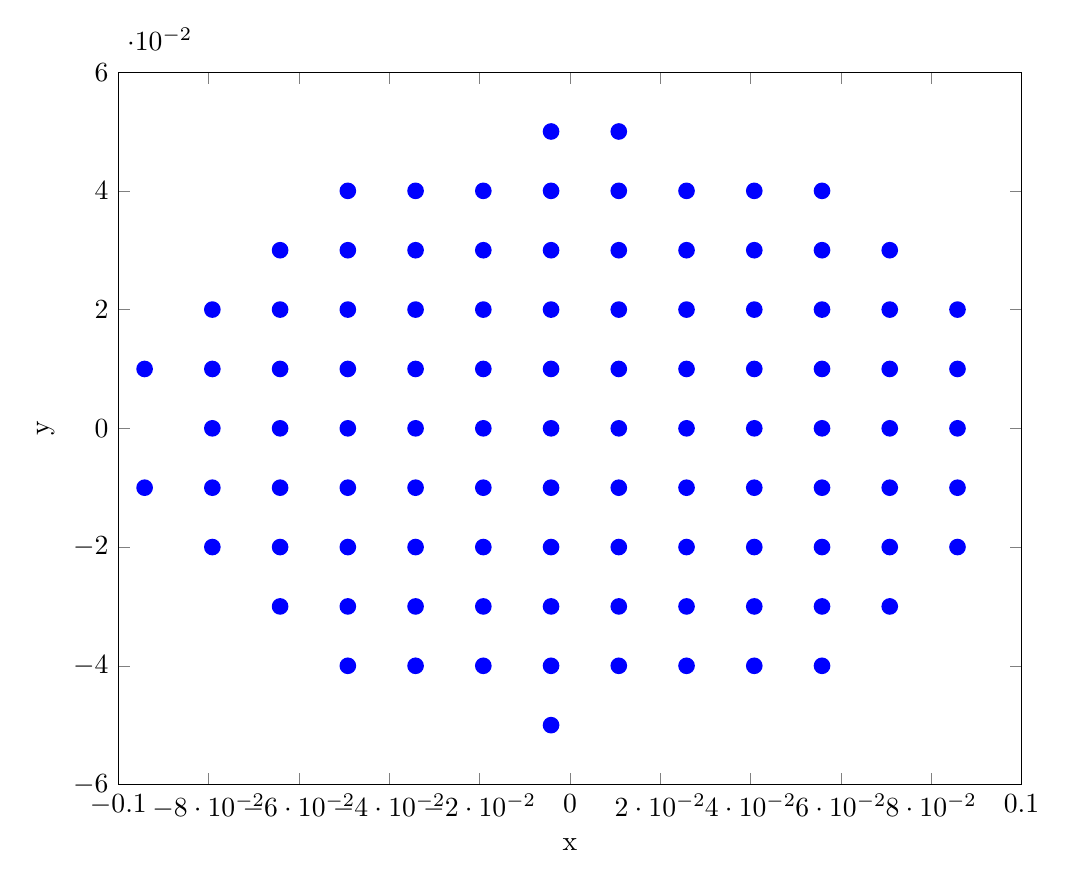
\begin{tikzpicture}

\begin{axis}[%
width=4.516in,
height=3.562in,
at={(0.758in,0.481in)},
scale only axis,
xmin=-0.1,
xmax=0.1,
xlabel={x},
ymin=-0.06,
ymax=0.06,
ylabel={y},
axis background/.style={fill=white}
]
\addplot [color=blue,line width=1.0pt,mark size=2.5pt,only marks,mark=*,mark options={solid},forget plot]
  table[row sep=crcr]{%
-0.0941809390575709	-0.01\\
-0.0941809390575709	0.00999999999999999\\
-0.0791809390575709	-0.02\\
-0.0791809390575709	-0.01\\
-0.0791809390575709	-1.04083408558608e-17\\
-0.0791809390575709	0.00999999999999999\\
-0.0791809390575709	0.02\\
-0.0641809390575709	-0.03\\
-0.0641809390575709	-0.02\\
-0.0641809390575709	-0.01\\
-0.0641809390575709	-1.04083408558608e-17\\
-0.0641809390575709	0.00999999999999999\\
-0.0641809390575709	0.02\\
-0.0641809390575709	0.03\\
-0.0491809390575709	-0.04\\
-0.0491809390575709	-0.03\\
-0.0491809390575709	-0.02\\
-0.0491809390575709	-0.01\\
-0.0491809390575709	-1.04083408558608e-17\\
-0.0491809390575709	0.00999999999999999\\
-0.0491809390575709	0.02\\
-0.0491809390575709	0.03\\
-0.0491809390575709	0.04\\
-0.0341809390575709	-0.04\\
-0.0341809390575709	-0.03\\
-0.0341809390575709	-0.02\\
-0.0341809390575709	-0.01\\
-0.0341809390575709	-1.04083408558608e-17\\
-0.0341809390575709	0.00999999999999999\\
-0.0341809390575709	0.02\\
-0.0341809390575709	0.03\\
-0.0341809390575709	0.04\\
-0.0191809390575709	-0.04\\
-0.0191809390575709	-0.03\\
-0.0191809390575709	-0.02\\
-0.0191809390575709	-0.01\\
-0.0191809390575709	-1.04083408558608e-17\\
-0.0191809390575709	0.00999999999999999\\
-0.0191809390575709	0.02\\
-0.0191809390575709	0.03\\
-0.0191809390575709	0.04\\
-0.00418093905757092	-0.05\\
-0.00418093905757092	-0.04\\
-0.00418093905757092	-0.03\\
-0.00418093905757092	-0.02\\
-0.00418093905757092	-0.01\\
-0.00418093905757092	-1.04083408558608e-17\\
-0.00418093905757092	0.00999999999999999\\
-0.00418093905757092	0.02\\
-0.00418093905757092	0.03\\
-0.00418093905757092	0.04\\
-0.00418093905757092	0.05\\
0.0108190609424291	-0.04\\
0.0108190609424291	-0.03\\
0.0108190609424291	-0.02\\
0.0108190609424291	-0.01\\
0.0108190609424291	-1.04083408558608e-17\\
0.0108190609424291	0.00999999999999999\\
0.0108190609424291	0.02\\
0.0108190609424291	0.03\\
0.0108190609424291	0.04\\
0.0108190609424291	0.05\\
0.0258190609424291	-0.04\\
0.0258190609424291	-0.03\\
0.0258190609424291	-0.02\\
0.0258190609424291	-0.01\\
0.0258190609424291	-1.04083408558608e-17\\
0.0258190609424291	0.00999999999999999\\
0.0258190609424291	0.02\\
0.0258190609424291	0.03\\
0.0258190609424291	0.04\\
0.0408190609424291	-0.04\\
0.0408190609424291	-0.03\\
0.0408190609424291	-0.02\\
0.0408190609424291	-0.01\\
0.0408190609424291	-1.04083408558608e-17\\
0.0408190609424291	0.00999999999999999\\
0.0408190609424291	0.02\\
0.0408190609424291	0.03\\
0.0408190609424291	0.04\\
0.0558190609424291	-0.04\\
0.0558190609424291	-0.03\\
0.0558190609424291	-0.02\\
0.0558190609424291	-0.01\\
0.0558190609424291	-1.04083408558608e-17\\
0.0558190609424291	0.00999999999999999\\
0.0558190609424291	0.02\\
0.0558190609424291	0.03\\
0.0558190609424291	0.04\\
0.0708190609424291	-0.03\\
0.0708190609424291	-0.02\\
0.0708190609424291	-0.01\\
0.0708190609424291	-1.04083408558608e-17\\
0.0708190609424291	0.00999999999999999\\
0.0708190609424291	0.02\\
0.0708190609424291	0.03\\
0.0858190609424291	-0.02\\
0.0858190609424291	-0.01\\
0.0858190609424291	-1.04083408558608e-17\\
0.0858190609424291	0.00999999999999999\\
0.0858190609424291	0.02\\
};
\end{axis}
\end{tikzpicture}%
    }
    \caption{Feasible positions of the body CoM at $c_{d}^{z} = 0.75 \MT{[m]}$
    with fixed arms and head.}
    \label{fig-kinematic-feasibility}
\end{figure}



%%%%%%%%%%%%%%%%%%%%%%%%%%%%%%%%%%%%%%%%%%%%%%%%%%%%%%%%%%%%%%%%%%%%%%%%%%%%%%%%%%%%%%%%%%%%%%%%%%%%%%
%%%%%%%%%%%%%%%%%%%%%%%%%%%%%%%%%%%%%%%%%%%%%%%%%%%%%%%%%%%%%%%%%%%%%%%%%%%%%%%%%%%%%%%%%%%%%%%%%%%%%%
%%%%%%%%%%%%%%%%%%%%%%%%%%%%%%%%%%%%%%%%%%%%%%%%%%%%%%%%%%%%%%%%%%%%%%%%%%%%%%%%%%%%%%%%%%%%%%%%%%%%%%
\clearpage
\section{Basic version}
Control variables
%
\begin{equation}
    \V{u}_k = \cjerk_k = (\cjbase[,k]^{x}, \cjbody[,k]^{x}, \cjbase[,k]^{y}, \cjbody[,k]^{y})
\end{equation}
%


%%%%%%%%%%%%%%%%%%%%%%%%%%%%%%%%%%%%%%%%%%%%%%%%%%%%%%%%%%%%%%%%%%%%%%%%%%%%%%%%%%%%%%%%%%%%%%%%%%%%%%
\subsection{Model}

\begin{align}
    \cstate_{k+1} &= \M{A}_k \cstate_{k} + \M{B}_k \V{u}_k\\
    \cop_{k} &= \M{D}_{p,k} \cstate_{k}
\end{align}

Four independent triple integrators (x, y motions of base and body)

%
\begin{equation}
    \M{A}_k = \diag{4}{
        \begin{bmatrix}
            1       & T_k   & T_k^2/2\\
            0       & 1     & T_k    \\
            0       & 0     & 1      \\
        \end{bmatrix}
    }
    , \quad
    \M{B}_k = \diag{4}{
        \begin{bmatrix}
            T_k^3/6\\
            T_k^2/2\\
            T      \\
        \end{bmatrix}
    }
\end{equation}
%
%
\begin{equation}
    \M{D}_{p,k} =
    \frac{1}{m_s + m_d}
    \diag{2}
    {
        \begin{bmatrix}
            {m_s}
            \begin{bmatrix}
                1       & 0     & - \frac{c^z_{s,k}}{g} \\
            \end{bmatrix}
            &
            {m_d}
            \begin{bmatrix}
                1       & 0     & - \frac{c^z_{d,k}}{g} \\
            \end{bmatrix}
        \end{bmatrix}
    }
\end{equation}
%


%%%%%%%%%%%%%%%%%%%%%%%%%%%%%%%%%%%%%%%%%%%%%%%%%%%%%%%%%%%%%%%%%%%%%%%%%%%%%%%%%%%%%%%%%%%%%%%%%%%%%%
\subsection{Constraints}

%%%%%%%%%%%%%%%%%%%%%%%%%%%%%%%%%%%%%%%%%%%%%%
\subsubsection{CoP}
Position
%
\begin{equation}
    \NORME{\cop - \cbase} \le r_s
\end{equation}
%

Approximated with a rectangle
%
\begin{equation}
    \underbrace{
        - \sqrt{2} r_s
        \begin{bmatrix}
            1\\
            1
        \end{bmatrix}
    }_{\ubarV{p}}
    \le
    \cop - \cbase
    \le
    \underbrace{
        \sqrt{2} r_s
        \begin{bmatrix}
            1\\
            1
        \end{bmatrix}
    }_{\barV{p}}
\end{equation}
%

Over the preview horizon
%
\begin{equation}
    \V{1}_N
    \kron
    \ubarV{p}
    \le
    \left(
        \diag{k = 1...N}{\M{D}_{p,k}} - \M{S}_{\cbase}
    \right)
    \left(
        \M{U}_x \cstate_0 + \M{U}_u \V{\Upsilon}
    \right)
    \le
    \V{1}_N
    \kron
    \barV{p}
\end{equation}
%


%%%%%%%%%%%%%%%%%%%%%%%%%%%%%%%%%%%%%%%%%%%%%%
\subsubsection{Base velocity}
%
\begin{equation}
    \NORME{\cvbase} \le \bar{v}
\end{equation}
%

Approximated with a rectangle
%
\begin{equation}
    \underbrace{
        - \sqrt{2} \bar{v}
        \begin{bmatrix}
            1\\
            1
        \end{bmatrix}
    }_{\ubarV{v}}
    \le
    \cvbase
    \le
    \underbrace{
        \sqrt{2} \bar{v}
        \begin{bmatrix}
            1\\
            1
        \end{bmatrix}
    }_{\barV{v}}
\end{equation}
%

Over the preview horizon
%
\begin{equation}
    \V{1}_N
    \kron
    \ubarV{v}
    \le
    \M{S}_{\cvbase}
    \left(
        \M{U}_x \cstate_0 + \M{U}_u \V{\Upsilon}
    \right)
    \le
    \V{1}_N
    \kron
    \barV{v}
\end{equation}
%

%%%%%%%%%%%%%%%%%%%%%%%%%%%%%%%%%%%%%%%%%%%%%%
\subsubsection{Base acceleration}
%
\begin{equation}
    \NORME{\cabase} \le \bar{a}
\end{equation}
%

Approximated with a rectangle
%
\begin{equation}
    \underbrace{
        - \sqrt{2} \bar{a}
        \begin{bmatrix}
            1\\
            1
        \end{bmatrix}
    }_{\ubarV{a}}
    \le
    \cabase
    \le
    \underbrace{
        \sqrt{2} \bar{a}
        \begin{bmatrix}
            1\\
            1
        \end{bmatrix}
    }_{\barV{a}}
\end{equation}
%

Over the preview horizon
%
\begin{equation}
    \V{1}_N
    \kron
    \ubarV{a}
    \le
    \M{S}_{\cabase}
    \left(
        \M{U}_x \cstate_0 + \M{U}_u \V{\Upsilon}
    \right)
    \le
    \V{1}_N
    \kron
    \barV{a}
\end{equation}
%


%%%%%%%%%%%%%%%%%%%%%%%%%%%%%%%%%%%%%%%%%%%%%%
\subsubsection{Body position}

Position with respect to the base
%
\begin{equation}
    \ubarV{d} \le \M[][S]{R} (\cbase - \cbody) \le \barV{d}
\end{equation}
%

Over the preview horizon
%
\begin{equation}
    \V{1}_N
    \kron
    \ubarV{d}
    \le
    \diag{k = 1...N}{\M[][S_k]{R}}
    \left(
        \M{S}_{\cbase} - \M{S}_{\cbody}
    \right)
    \left(
        \M{U}_x \cstate_0 + \M{U}_u \V{\Upsilon}
    \right)
    \le
    \V{1}_N
    \kron
    \barV{d}
\end{equation}
%


%%%%%%%%%%%%%%%%%%%%%%%%%%%%%%%%%%%%%%%%%%%%%%%%%%%%%%%%%%%%%%%%%%%%%%%%%%%%%%%%%%%%%%%%%%%%%%%%%%%%%%
\subsection{Objective function}

%%%%%%%%%%%%%%%%%%%%%%%%%%%%%%%%%%
\subsubsection{Base position}
\begin{equation}
    \M{S}_{\cbase}
    \left(
        \M{U}_x \cstate_0 + \M{U}_u \V{\Upsilon}
    \right)
    -
    (\cBase)_{\MT{ref}}
    =
    \V{0}
\end{equation}


%%%%%%%%%%%%%%%%%%%%%%%%%%%%%%%%%%
\subsubsection{Velocity}
\begin{equation}
    \M{S}_{\cvbase}
    \left(
        \M{U}_x \cstate_0 + \M{U}_u \V{\Upsilon}
    \right)
    -
    (\cvBase)_{\MT{ref}}
    =
    \V{0}
\end{equation}


%%%%%%%%%%%%%%%%%%%%%%%%%%%%%%%%%%
\subsubsection{Jerk (simple)}
\begin{equation}
    \V{\Upsilon}
    =
    \V{0}
\end{equation}


%%%%%%%%%%%%%%%%%%%%%%%%%%%%%%%%%%
\subsubsection{CoP}
\begin{equation}
    \left(
        \diag{k = 1...N}{\M{D}_{p,k}} - \M{S}_{\cbase}
    \right)
    \left(
        \M{U}_x \cstate_0 + \M{U}_u \V{\Upsilon}
    \right)
    =
    \V{0}
\end{equation}


%%%%%%%%%%%%%%%%%%%%%%%%%%%%%%%%%%
\subsubsection{Body position}
\begin{equation}
    \left(
        \M{S}_{\cbase} - \M{S}_{\cbody}
    \right)
    \left(
        \M{U}_x \cstate_0 + \M{U}_u \V{\Upsilon}
    \right)
    =
    \V{0}
\end{equation}


%%%%%%%%%%%%%%%%%%%%%%%%%%%%%%%%%%%%%%%%%%%%%%%%%%%%%%%%%%%%%%%%%%%%%%%%%%%%%%%%%%%%%%%%%%%%%%%%%%%%%%
\subsection{Changing output variables}
Instead of $\cop_k$ we can directly compute
%
\begin{equation}
    \cop[S_k]
    =
    \cop_k - \cbase[,k]
\end{equation}
%
as the output of the system. Since this difference is constrained to a circle
(approximated), orientation of the base is not important.

\begin{align}
    \M{D}_{p,k}
    &=
        \frac{1}{m_s + m_d}
        \diag{2}
        {
            \begin{bmatrix}
                {m_s}
                \begin{bmatrix}
                    1       & 0     & - \frac{c^z_{s,k}}{g} \\
                \end{bmatrix}
                &
                {m_d}
                \begin{bmatrix}
                    1       & 0     & - \frac{c^z_{d,k}}{g} \\
                \end{bmatrix}
            \end{bmatrix}
        }
        \\
    &=
        \frac{1}{m_s + m_d}
        \diag{2}
        {
            \begin{bmatrix}
                {m_s}       & 0     & - \frac{c^z_{s,k}}{g}{m_s}
                &
                {m_d}       & 0     & - \frac{c^z_{d,k}}{g}{m_d} \\
            \end{bmatrix}
        }
\end{align}
%

%
\begin{align}
    \M{S}_{\cbase,k}
    &=
        \diag{2}{
            \begin{bmatrix}
                1 & 0 & 0 & 0 & 0 & 0\\
            \end{bmatrix}
        }
        \\
    &=
        \frac{1}{m_s + m_d}
        \diag{2}{
            \begin{bmatrix}
                {m_s + m_d} & 0 & 0 & 0 & 0 & 0\\
            \end{bmatrix}
        }
\end{align}
%

%
\begin{align}
    \M{D}_{ps,k}
    &=
        \M{D}_{p,k}
        -
        \M{S}_{\cbase,k}
        \\
    &=
        \frac{1}{m_s + m_d}
        \diag{2}
        {
            \begin{bmatrix}
                -{m_d}      & 0     & - \frac{c^z_{s,k}}{g}{m_s}
                &
                {m_d}       & 0     & - \frac{c^z_{d,k}}{g}{m_d} \\
            \end{bmatrix}
        }
\end{align}
%




%%%%%%%%%%%%%%%%%%%%%%%%%%%%%%%%%%%%%%%%%%%%%%%%%%%%%%%%%%%%%%%%%%%%%%%%%%%%%%%%%%%%%%%%%%%%%%%%%%%%%%
%%%%%%%%%%%%%%%%%%%%%%%%%%%%%%%%%%%%%%%%%%%%%%%%%%%%%%%%%%%%%%%%%%%%%%%%%%%%%%%%%%%%%%%%%%%%%%%%%%%%%%
%%%%%%%%%%%%%%%%%%%%%%%%%%%%%%%%%%%%%%%%%%%%%%%%%%%%%%%%%%%%%%%%%%%%%%%%%%%%%%%%%%%%%%%%%%%%%%%%%%%%%%
\clearpage
\section{With simple bounds (Version 1: base velocity)}

Control variables
%
\begin{equation}
    \V{u}_k = (\cvbase[,k+1]^{x}, \cjbody[,k]^{x}, \cvbase[,k+1]^{y}, \cjbody[,k]^{y})
\end{equation}
%

%%%%%%%%%%%%%%%%%%%%%%%%%%%%%%%%%%%%%%%%%%%%%%%%%%%%%%%%%%%%%%%%%%%%%%%%%%%%%%%%%%%%%%%%%%%%%%%%%%%%%%
\subsection{Model}

\begin{align}
    \cstate_{k+1}   &= \M{A}_k \cstate_{k} + \M{B}_k \V{u}_k\\
    \cop[S_k]_{k}   &= \M{D}_{ps,k} \cstate_{k} \\
    \cjbase[,k]     &= \M{D}_{\cjerk,k} \cstate_{k} + \M{E}_{\cjerk,k} \V{u}_{k}
\end{align}

Four independent triple integrators (x, y motions of base and body), triple
integrators corresponding to base motion are controlled with velocities.

%
\begin{equation}
    \M{A}_k = \diag{2}{
        \diag{}{
            \begin{bmatrix}
                1     & \frac{2 T_k}{3}     & \frac{T_k^2}{6} \\
                0     & 0                   & 0 \\
                0     & -\frac{2}{T_k}      &  - 1 \\
            \end{bmatrix}
            ,
            \begin{bmatrix}
                1       & T_k   & T_k^2/2\\
                0       & 1     & T_k    \\
                0       & 0     & 1      \\
            \end{bmatrix}
        }
    }
\end{equation}
%

%
\begin{equation}
    \M{B}_k = \diag{2}{
        \diag{}{
            \begin{bmatrix}
                \frac{T_k}{3} \\
                1 \\
                \frac{2}{T_k} \\
            \end{bmatrix}
            ,
            \begin{bmatrix}
                T_k^3/6\\
                T_k^2/2\\
                T      \\
            \end{bmatrix}
        }
    }
\end{equation}
%

%
\begin{equation}
    \M{D}_{ps,k}
    =
        \frac{1}{m_s + m_d}
        \diag{2}
        {
            \begin{bmatrix}
                -{m_d}      & 0     & - \frac{c^z_{s,k}}{g}{m_s}
                &
                {m_d}       & 0     & - \frac{c^z_{d,k}}{g}{m_d} \\
            \end{bmatrix}
        }
\end{equation}
%

%
\begin{equation}
    \M{D}_{\cjerk,k} =
    \diag{2}{
        \begin{bmatrix}
            \begin{bmatrix}
                0 & -\frac{2}{T_k^2} & -\frac{2}{T_k}\\
            \end{bmatrix}
            &
            \begin{bmatrix}
                0       & 0     & 0 \\
            \end{bmatrix}
        \end{bmatrix}
    },
    \quad
    \M{E}_{\cjerk,k} =
    \diag{2}{
        \begin{bmatrix}
            \begin{bmatrix}
                \frac{2}{T_k^2} \\
            \end{bmatrix}
            &
            \begin{bmatrix}
                0  \\
            \end{bmatrix}
        \end{bmatrix}
    },
\end{equation}
%


%%%%%%%%%%%%%%%%%%%%%%%%%%%%%%%%%%%%%%%%%%%%%%%%%%%%%%%%%%%%%%%%%%%%%%%%%%%%%%%%%%%%%%%%%%%%%%%%%%%%%%
\subsection{Constraints}

%%%%%%%%%%%%%%%%%%%%%%%%%%%%%%%%%%%%%%%%%%%%%%
\subsubsection{CoP}
Position
%
\begin{equation}
    \NORME{\cop[S]} \le r_s
\end{equation}
%

Approximated with a rectangle
%
\begin{equation}
    \underbrace{
        - \sqrt{2} r_s
        \begin{bmatrix}
            1\\
            1
        \end{bmatrix}
    }_{\ubarV{p}}
    \le
    \cop[S]
    \le
    \underbrace{
        \sqrt{2} r_s
        \begin{bmatrix}
            1\\
            1
        \end{bmatrix}
    }_{\barV{p}}
\end{equation}
%

Over the preview horizon
%
\begin{equation}
    \V{1}_N
    \kron
    \ubarV{p}
    \le
    \diag{k = 1...N}{\M{D}_{ps,k}}
    \left(
        \M{U}_x \cstate_0 + \M{U}_u \V{\Upsilon}
    \right)
    \le
    \V{1}_N
    \kron
    \barV{p}
\end{equation}
%


%%%%%%%%%%%%%%%%%%%%%%%%%%%%%%%%%%%%%%%%%%%%%%
\subsubsection{Base velocity (simple bounds)}
%
\begin{equation}
    \NORME{\cvbase} \le \bar{v}
\end{equation}
%

Approximated with a rectangle
%
\begin{equation}
    \underbrace{
        - \sqrt{2} \bar{v}
        \begin{bmatrix}
            1\\
            1
        \end{bmatrix}
    }_{\ubarV{v}}
    \le
    \cvbase
    \le
    \underbrace{
        \sqrt{2} \bar{v}
        \begin{bmatrix}
            1\\
            1
        \end{bmatrix}
    }_{\barV{v}}
\end{equation}
%

Over the preview horizon
%
\begin{equation}
    \V{1}_N
    \kron
    \ubarV{v}
    \le
    \M{S}_{\cvbase}
    \V{\Upsilon}
    \le
    \V{1}_N
    \kron
    \barV{v}
\end{equation}
%


%%%%%%%%%%%%%%%%%%%%%%%%%%%%%%%%%%%%%%%%%%%%%%
\subsubsection{Base acceleration}
%
\begin{equation}
    \NORME{\cabase} \le \bar{a}
\end{equation}
%

Approximated with a rectangle
%
\begin{equation}
    \underbrace{
        - \sqrt{2} \bar{a}
        \begin{bmatrix}
            1\\
            1
        \end{bmatrix}
    }_{\ubarV{a}}
    \le
    \cabase
    \le
    \underbrace{
        \sqrt{2} \bar{a}
        \begin{bmatrix}
            1\\
            1
        \end{bmatrix}
    }_{\barV{a}}
\end{equation}
%

Over the preview horizon
%
\begin{equation}
    \V{1}_N
    \kron
    \ubarV{a}
    \le
    \M{S}_{\cabase}
    \left(
        \M{U}_x \cstate_0 + \M{U}_u \V{\Upsilon}
    \right)
    \le
    \V{1}_N
    \kron
    \barV{a}
\end{equation}
%


%%%%%%%%%%%%%%%%%%%%%%%%%%%%%%%%%%%%%%%%%%%%%%
\subsubsection{Body position}

Position with respect to the base
%
\begin{equation}
    \ubarV{d} \le \M[][S]{R} (\cbase - \cbody) \le \barV{d}
\end{equation}
%

Over the preview horizon
%
\begin{equation}
    \V{1}_N
    \kron
    \ubarV{d}
    \le
    \diag{k = 1...N}{\M[][S_k]{R}}
    \left(
        \M{S}_{\cbase} - \M{S}_{\cbody}
    \right)
    \left(
        \M{U}_x \cstate_0 + \M{U}_u \V{\Upsilon}
    \right)
    \le
    \V{1}_N
    \kron
    \barV{d}
\end{equation}
%


%%%%%%%%%%%%%%%%%%%%%%%%%%%%%%%%%%%%%%%%%%%%%%%%%%%%%%%%%%%%%%%%%%%%%%%%%%%%%%%%%%%%%%%%%%%%%%%%%%%%%%
\subsection{Objective function}

%%%%%%%%%%%%%%%%%%%%%%%%%%%%%%%%%%%%%%
\subsubsection{Base position}
\begin{equation}
    \M{S}_{\cbase}
    \left(
        \M{U}_x \cstate_0 + \M{U}_u \V{\Upsilon}
    \right)
    -
    (\cBase)_{\MT{ref}}
    =
    \V{0}
\end{equation}



%%%%%%%%%%%%%%%%%%%%%%%%%%%%%%%%%%%%%%
\subsubsection{Velocity (simple)}
\begin{equation}
    \M{S}_{\cvbase}
    \V{\Upsilon}
    -
    (\cvBase)_{\MT{ref}}
    =
    \V{0}
\end{equation}



%%%%%%%%%%%%%%%%%%%%%%%%%%%%%%%%%%%%%%
\subsubsection{Jerk (partially simple)}
\begin{equation}
    \M{S}_{\cjbody}
    \V{\Upsilon}
    =
    \V{0}
\end{equation}

\begin{equation}
    \M{O}_{\cjerk,x}
    \cstate_0
    +
    \M{O}_{\cjerk,u}
    \V{\Upsilon}
    =
    \V{0}
\end{equation}



%%%%%%%%%%%%%%%%%%%%%%%%%%%%%%%%%%%%%%
\subsubsection{CoP}
\begin{equation}
    \diag{k = 1...N}{\M{D}_{p,k}}
    \left(
        \M{U}_x \cstate_0 + \M{U}_u \V{\Upsilon}
    \right)
    =
    \V{0}
\end{equation}



%%%%%%%%%%%%%%%%%%%%%%%%%%%%%%%%%%%%%%
\subsubsection{Body position}
\begin{equation}
    \left(
        \M{S}_{\cbase} - \M{S}_{\cbody}
    \right)
    \left(
        \M{U}_x \cstate_0 + \M{U}_u \V{\Upsilon}
    \right)
    =
    \V{0}
\end{equation}



%%%%%%%%%%%%%%%%%%%%%%%%%%%%%%%%%%%%%%%%%%%%%%%%%%%%%%%%%%%%%%%%%%%%%%%%%%%%%%%%%%%%%%%%%%%%%%%%%%%%%%
%%%%%%%%%%%%%%%%%%%%%%%%%%%%%%%%%%%%%%%%%%%%%%%%%%%%%%%%%%%%%%%%%%%%%%%%%%%%%%%%%%%%%%%%%%%%%%%%%%%%%%
%%%%%%%%%%%%%%%%%%%%%%%%%%%%%%%%%%%%%%%%%%%%%%%%%%%%%%%%%%%%%%%%%%%%%%%%%%%%%%%%%%%%%%%%%%%%%%%%%%%%%%
\clearpage
\section{With simple bounds (Version 1 + sparsity and variable separation)}

State variables
\begin{align}
    \cstate_s &= ({c}^x_s, \dot{c}^x_s, \ddot{c}^x_s, {c}^y_s, \dot{c}^y_s, \ddot{c}^y_s)\\
    \cstate_d &= ({c}^x_d, \dot{c}^x_d, \ddot{c}^x_d, {c}^y_d, \dot{c}^y_d, \ddot{c}^y_d)
\end{align}

Control variables
%
\begin{align}
    \V{u}_{s,k} &= (\cvbase[,k+1]^{x}, \cvbase[,k+1]^{y})\\
    \V{u}_{d,k} &= (\cjbody[,k]^{x}, \cjbody[,k]^{y})
\end{align}
%


%%%%%%%%%%%%%%%%%%%%%%%%%%%%%%%%%%%%%%%%%%%%%%%%%%%%%%%%%%%%%%%%%%%%%%%%%%%%%%%%%%%%%%%%%%%%%%%%%%%%%%
\subsection{Model}

\begin{align}
    \cstate_{s,k+1}   &= \M{A}_{s,k} \cstate_{s,k} + \M{B}_{s,k} \V{u}_{s,k}\\
    \cstate_{d,k+1}   &= \M{A}_{d,k} \cstate_{d,k} + \M{B}_{d,k} \V{u}_{d,k}\\
    \cop[S_k]_{k}   &= \M{D}_{\MT{ps},s,k} \cstate_{s,k} + \M{D}_{\MT{ps},d,k} \cstate_{d,k}\\
    \cjbase[,k]    &= \M{D}_{\cjerk,s,k} \cstate_{k} + \M{E}_{\cjerk,s,k} \V{u}_{s,k}
\end{align}

Four independent triple integrators (x, y motions of base and body), triple
integrators corresponding to base motion are controlled with velocities.

%
\begin{equation}
    \M{A}_{s,k} =
        \M{I}_2
        \kron
        \M{A}_{s,k}^{\MT{x|y}}
    ,
    \quad
    \M{A}_{d,k} =
        \M{I}_2
        \kron
        \M{A}_{d,k}^{\MT{x|y}}
    ,
    \quad
    \M{B}_{s,k} =
        \M{I}_2
        \kron
        \M{B}_{s,k}^{\MT{x|y}}
    ,
    \quad
    \M{B}_{d,k} =
        \M{I}_2
        \kron
        \M{B}_{d,k}^{\MT{x|y}}
\end{equation}
%

%
\begin{equation}
    \M{A}_{s,k}^{\MT{x|y}}
    =
        \begin{bmatrix}
            1     & \frac{2 T_k}{3}     & \frac{T_k^2}{6} \\
            0     & 0                   & 0 \\
            0     & -\frac{2}{T_k}      &  - 1 \\
        \end{bmatrix}
    ,
    \quad
    \M{A}_{d,k}^{\MT{x|y}}
    =
        \begin{bmatrix}
            1       & T_k   & T_k^2/2\\
            0       & 1     & T_k    \\
            0       & 0     & 1      \\
        \end{bmatrix}
\end{equation}
%

%
\begin{equation}
    \M{B}_{s,k}^{\MT{x|y}}
    =
        \begin{bmatrix}
            \frac{T_k}{3} \\
            1 \\
            \frac{2}{T_k} \\
        \end{bmatrix}
    ,
    \quad
    \M{B}_{d,k}^{\MT{x|y}}
    =
        \begin{bmatrix}
            T_k^3/6\\
            T_k^2/2\\
            T      \\
        \end{bmatrix}
\end{equation}
%

%
\begin{align}
    \M{D}_{\MT{ps},s,k}
    =
        \M{I}_2
        \kron
        \M{D}_{\MT{ps},s,k}^{\MT{x|y}}
    &=
        \M{I}_2
        \kron
        \left(
            \frac{1}{m_s + m_d}
            \begin{bmatrix}
                -{m_d}      & 0     & - \frac{c^z_{s,k}}{g}{m_s}
            \end{bmatrix}
        \right)
    ,
    \\
    \M{D}_{\MT{ps},d,k}
    =
        \M{I}_2
        \kron
        \M{D}_{\MT{ps},d,k}^{\MT{x|y}}
    &=
        \M{I}_2
        \kron
        \left(
            \frac{1}{m_s + m_d}
            \begin{bmatrix}
                {m_d}       & 0     & - \frac{c^z_{d,k}}{g}{m_d} \\
            \end{bmatrix}
        \right)
\end{align}
%

%
\begin{equation}
    \M{D}_{\cjerk,s,k}
    =
        \M{I}_2
        \kron
        \M{D}_{\cjerk,s,k}^{\MT{x|y}}
    =
        \M{I}_2
        \kron
        \begin{bmatrix}
            0 & -\frac{2}{T_k^2} & -\frac{2}{T_k}
        \end{bmatrix}
    ,
    \quad
    \M{E}_{\cjerk,s,k}
    =
        \M{I}_2
        \kron
        \M{E}_{\cjerk,s,k}^{\MT{x|y}}
    =
        \M{I}_2
        \kron
        \begin{bmatrix}
            \frac{2}{T_k^2}
        \end{bmatrix}
\end{equation}
%


%%%%%%%%%%%%%%%%%%%%%%%%%%%%%%%%%%%%%%%%%%%%%%%%%%%%%%%%%%%%%%%%%%%%%%%%%%%%%%%%%%%%%%%%%%%%%%%%%%%%%%
\subsection{Constraints}

%%%%%%%%%%%%%%%%%%%%%%%%%%%%%%%%%%%%%%%%%%%%%%
\subsubsection{CoP}
Position
%
\begin{equation}
    \NORME{\cop[S]} \le r_s
\end{equation}
%

Approximated with a rectangle
%
\begin{equation}
    \underbrace{
        - \sqrt{2} r_s
        \begin{bmatrix}
            1\\
            1
        \end{bmatrix}
    }_{\ubarV{p}}
    \le
    \cop[S]
    \le
    \underbrace{
        \sqrt{2} r_s
        \begin{bmatrix}
            1\\
            1
        \end{bmatrix}
    }_{\barV{p}}
\end{equation}
%

Over the preview horizon
%
\begin{equation}
    \begin{split}
        \V{1}_N
        \kron
        \ubarV{p}
        \le
        &
        \diag{k = 1...N}{\M{I}_2 \kron \M{D}_{\MT{ps},s,k}}
        \left(
            (\M{I}_2 \bkron \M{U}^{\MT{x|y}}_{s,x}) \cstate_{s,0}
            +
            (\M{I}_2 \bkron \M{U}^{\MT{x|y}}_{s,u}) \V{\Upsilon}_s
        \right)\\
        &
        +
        \diag{k = 1...N}{\M{I}_2 \kron \M{D}_{\MT{ps},d,k}}
        \left(
            (\M{I}_2 \bkron \M{U}^{\MT{x|y}}_{d,x}) \cstate_{d,0}
            +
            (\M{I}_2 \bkron \M{U}^{\MT{x|y}}_{d,u}) \V{\Upsilon}_d
        \right)
        \le
        \V{1}_N
        \kron
        \barV{p}
    \end{split}
\end{equation}
%
%
\begin{multline}
    \V{1}_N
    \kron
    \ubarV{p}
    -
    \diag{k = 1...N}{\M{I}_2 \kron \M{D}_{\MT{ps},s,k}}
    (\M{I}_2 \bkron \M{U}^{\MT{x|y}}_{s,x}) \cstate_{s,0}
    -
    \diag{k = 1...N}{\M{I}_2 \kron \M{D}_{\MT{ps},d,k}}
    (\M{I}_2 \bkron \M{U}^{\MT{x|y}}_{d,x}) \cstate_{d,0}
    \\
        \le
        \diag{k = 1...N}{\M{I}_2 \kron \M{D}_{\MT{ps},s,k}}
        (\M{I}_2 \bkron \M{U}^{\MT{x|y}}_{s,u}) \V{\Upsilon}_s
        +
        \diag{k = 1...N}{\M{D}_{\MT{ps},d,k}}
        (\M{I}_2 \bkron \M{U}^{\MT{x|y}}_{d,u}) \V{\Upsilon}_d
        \le
    \\
    \V{1}_N
    \kron
    \barV{p}
    -
    \diag{k = 1...N}{\M{I}_2 \kron \M{D}_{\MT{ps},s,k}}
    (\M{I}_2 \bkron \M{U}^{\MT{x|y}}_{s,x}) \cstate_{s,0}
    -
    \diag{k = 1...N}{\M{I}_2 \kron \M{D}_{\MT{ps},d,k}}
    (\M{I}_2 \bkron \M{U}^{\MT{x|y}}_{d,x}) \cstate_{d,0}
\end{multline}
%
%
\begin{multline}
    \V{1}_N
    \kron
    \ubarV{p}
    -
    \M{I}_2 \bkron
        (\diag{k = 1...N}{\M{D}_{\MT{ps},s,k}}
        \M{U}^{\MT{x|y}}_{s,x})
        \cstate_{s,0}
    -
    \M{I}_2 \bkron
        (\diag{k = 1...N}{\M{D}_{\MT{ps},d,k}}
        \M{U}^{\MT{x|y}}_{d,x})
        \cstate_{d,0}
    \\
        \le
        \begin{bmatrix}
            \M{I}_2 \bkron
                (\diag{k = 1...N}{\M{D}_{\MT{ps},s,k}}
                \M{U}^{\MT{x|y}}_{s,u})
                &
            \M{I}_2 \bkron
                (\diag{k = 1...N}{\M{D}_{\MT{ps},d,k}}
                \M{U}^{\MT{x|y}}_{d,u})
        \end{bmatrix}
        \V{\Upsilon}
        \le
    \\
    \V{1}_N
    \kron
    \barV{p}
    -
    \M{I}_2 \bkron
        (\diag{k = 1...N}{\M{D}_{\MT{ps},s,k}}
        \M{U}^{\MT{x|y}}_{s,x})
        \cstate_{s,0}
    -
    \M{I}_2 \bkron
        (\diag{k = 1...N}{\M{D}_{\MT{ps},d,k}}
        \M{U}^{\MT{x|y}}_{d,x})
        \cstate_{d,0}
\end{multline}
%


%%%%%%%%%%%%%%%%%%%%%%%%%%%%%%%%%%%%%%%%%%%%%%
\subsubsection{Base velocity (simple bounds)}
%
\begin{equation}
    \NORME{\cvbase} \le \bar{v}
\end{equation}
%

Approximated with a rectangle
%
\begin{equation}
    \underbrace{
        - \sqrt{2} \bar{v}
        \begin{bmatrix}
            1\\
            1
        \end{bmatrix}
    }_{\ubarV{v}}
    \le
    \cvbase
    \le
    \underbrace{
        \sqrt{2} \bar{v}
        \begin{bmatrix}
            1\\
            1
        \end{bmatrix}
    }_{\barV{v}}
\end{equation}
%

Over the preview horizon
%
\begin{equation}
    \V{1}_N
    \kron
    \ubarV{v}
    \le
    \V{\Upsilon}_s
    \le
    \V{1}_N
    \kron
    \barV{v}
\end{equation}
%


%%%%%%%%%%%%%%%%%%%%%%%%%%%%%%%%%%%%%%%%%%%%%%
\subsubsection{Base acceleration}
%
\begin{equation}
    \NORME{\cabase} \le \bar{a}
\end{equation}
%

Approximated with a rectangle
%
\begin{equation}
    \underbrace{
        - \sqrt{2} \bar{a}
        \begin{bmatrix}
            1\\
            1
        \end{bmatrix}
    }_{\ubarV{a}}
    \le
    \cabase
    \le
    \underbrace{
        \sqrt{2} \bar{a}
        \begin{bmatrix}
            1\\
            1
        \end{bmatrix}
    }_{\barV{a}}
\end{equation}
%

Over the preview horizon
%
\begin{equation}
    \V{1}_N
    \kron
    \ubarV{a}
    \le
    \M{S}_{\cabase}
    \left(
        (\M{I}_2 \bkron \M{U}^{\MT{x|y}}_{s,x}) \cstate_{s,0}
        +
        (\M{I}_2 \bkron \M{U}^{\MT{x|y}}_{s,u}) \V{\Upsilon}_s
    \right)
    \le
    \V{1}_N
    \kron
    \barV{a}
\end{equation}
%
%
\begin{equation}
    \M{S}_{\cabase}
    =
    \diag{N}{
        \M{I}_2
        \kron
        \begin{bmatrix}
            0 & 0 & 1
        \end{bmatrix}
    }
    =
    \M{I}_2
    \bkron
    \M{S}_{\cabase}^{\MT{x|y}}
\end{equation}
%
%
\begin{equation}
    \V{1}_N
    \kron
    \ubarV{a}
    \le
    (
        \M{I}_2
        \bkron
        \M{S}_{\cabase}^{\MT{x|y}}
    )
    \left(
        (\M{I}_2 \bkron \M{U}^{\MT{x|y}}_{s,x}) \cstate_{s,0}
        +
        (\M{I}_2 \bkron \M{U}^{\MT{x|y}}_{s,u}) \V{\Upsilon}_s
    \right)
    \le
    \V{1}_N
    \kron
    \barV{a}
\end{equation}
%
%
\begin{multline}
    \V{1}_N
    \kron
    \ubarV{a}
    -
    (
        \M{I}_2
        \bkron
        \M{S}_{\cabase}^{\MT{x|y}}
    )
    (\M{I}_2 \bkron \M{U}^{\MT{x|y}}_{s,x}) \cstate_{s,0}
    \\
        \le
        (
            \M{I}_2
            \bkron
            \M{S}_{\cabase}^{\MT{x|y}}
        )
        (\M{I}_2 \bkron \M{U}^{\MT{x|y}}_{s,u}) \V{\Upsilon}_s
        \le
    \\
    \V{1}_N
    \kron
    \barV{a}
    -
    (
        \M{I}_2
        \bkron
        \M{S}_{\cabase}^{\MT{x|y}}
    )
    (\M{I}_2 \bkron \M{U}^{\MT{x|y}}_{s,x}) \cstate_{s,0}
\end{multline}
%
%
\begin{multline}
    \V{1}_N
    \kron
    \ubarV{a}
    -
    \M{I}_2
    \bkron
    (
        \M{S}_{\cabase}^{\MT{x|y}}
        \M{U}^{\MT{x|y}}_{s,x}
    ) \cstate_{s,0}
    \\
        \le
        \M{I}_2
        \bkron
        (
            \M{S}_{\cabase}^{\MT{x|y}}
            \M{U}^{\MT{x|y}}_{s,u}
        ) \V{\Upsilon}_s
        \le
    \\
    \V{1}_N
    \kron
    \barV{a}
    -
    \M{I}_2
    \bkron
    (
        \M{S}_{\cabase}^{\MT{x|y}}
        \M{U}^{\MT{x|y}}_{s,x}
    ) \cstate_{s,0}
\end{multline}
%


%%%%%%%%%%%%%%%%%%%%%%%%%%%%%%%%%%%%%%%%%%%%%%
\subsubsection{Body position}

Position with respect to the base
%
\begin{equation}
    \ubarV{d} \le \M[][S]{R} (\cbase - \cbody) \le \barV{d}
\end{equation}
%

Over the preview horizon
%
\begin{equation}
    \begin{split}
        \V{1}_N
        \kron
        \ubarV{d}
            \le
            \diag{k = 1...N}{\M[][S_k]{R}}
            \Bigg(
                &
                \M{S}_{\V{c}}
                \left(
                    (\M{I}_2 \bkron \M{U}^{\MT{x|y}}_{s,x}) \cstate_{s,0}
                    +
                    (\M{I}_2 \bkron \M{U}^{\MT{x|y}}_{s,u}) \V{\Upsilon}_s
                \right)
                \\
                &
                -
                \M{S}_{\V{c}}
                \left(
                    (\M{I}_2 \bkron \M{U}^{\MT{x|y}}_{d,x}) \cstate_{d,0}
                    +
                    (\M{I}_2 \bkron \M{U}^{\MT{x|y}}_{d,u}) \V{\Upsilon}_d
                \right)
            \Bigg)
            \le
        \V{1}_N
        \kron
        \barV{d}
    \end{split}
\end{equation}
%
%
\begin{equation}
    \M{S}_{\V{c}}
    =
    \diag{N}{
        \M{I}_2
        \kron
        \begin{bmatrix}
            1 & 0 & 0
        \end{bmatrix}
    }
    =
    \M{I}_2
    \bkron
    \M{S}_{\V{c}}^{\MT{x|y}}
\end{equation}
%
%
\begin{equation}
    \begin{split}
        \V{1}_N
        \kron
        \ubarV{d}
            \le
            \diag{k = 1...N}{\M[][S_k]{R}}
            \Bigg(
                &
                \M{I}_2 \bkron (\M{S}_{\V{c}}^{\MT{x|y}} \M{U}^{\MT{x|y}}_{s,x}) \cstate_{s,0}
                +
                \M{I}_2 \bkron (\M{S}_{\V{c}}^{\MT{x|y}} \M{U}^{\MT{x|y}}_{s,u}) \V{\Upsilon}_s
                \\
            &
                -
                \M{I}_2 \bkron (\M{S}_{\V{c}}^{\MT{x|y}} \M{U}^{\MT{x|y}}_{d,x}) \cstate_{d,0}
                -
                \M{I}_2 \bkron (\M{S}_{\V{c}}^{\MT{x|y}} \M{U}^{\MT{x|y}}_{d,u}) \V{\Upsilon}_d
            \Bigg)
            \le
        \V{1}_N
        \kron
        \barV{d}
    \end{split}
\end{equation}
%
%
\begin{multline}
    \V{1}_N
    \kron
    \ubarV{d}
    -
    \diag{k = 1...N}{\M[][S_k]{R}}
    \left(
        \M{I}_2 \bkron (\M{S}_{\V{c}}^{\MT{x|y}} \M{U}^{\MT{x|y}}_{s,x})
        \cstate_{s,0}
        -
        \M{I}_2 \bkron (\M{S}_{\V{c}}^{\MT{x|y}} \M{U}^{\MT{x|y}}_{d,x})
        \cstate_{d,0}
    \right)
    \le
    \\
        \begin{bmatrix}
            \diag{k = 1...N}{\M[][S_k]{R}}
            \left(
                \M{I}_2 \bkron (\M{S}_{\V{c}}^{\MT{x|y}} \M{U}^{\MT{x|y}}_{s,u})
            \right)
            &
            -
            \diag{k = 1...N}{\M[][S_k]{R}}
            \left(
                \M{I}_2 \bkron (\M{S}_{\V{c}}^{\MT{x|y}} \M{U}^{\MT{x|y}}_{d,u})
            \right)
        \end{bmatrix}
        \V{\Upsilon}
    \\
    \le
    \V{1}_N
    \kron
    \barV{d}
    -
    \diag{k = 1...N}{\M[][S_k]{R}}
    \left(
        \M{I}_2 \bkron (\M{S}_{\V{c}}^{\MT{x|y}} \M{U}^{\MT{x|y}}_{s,x})
        \cstate_{s,0}
        -
        \M{I}_2 \bkron (\M{S}_{\V{c}}^{\MT{x|y}} \M{U}^{\MT{x|y}}_{d,x})
        \cstate_{d,0}
    \right)
\end{multline}
%


%%%%%%%%%%%%%%%%%%%%%%%%%%%%%%%%%%%%%%%%%%%%%%%%%%%%%%%%%%%%%%%%%%%%%%%%%%%%%%%%%%%%%%%%%%%%%%%%%%%%%%
\subsection{Objective function}

%%%%%%%%%%%%%%%%%%%%%%%%%%%%%%%%%%%%%%
\subsubsection{Base position}
%
\begin{equation}
    \M{I}_2 \bkron (\M{S}_{\V{c}}^{\MT{x|y}} \M{U}^{\MT{x|y}}_{s,x}) \cstate_{s,0}
    +
    \M{I}_2 \bkron (\M{S}_{\V{c}}^{\MT{x|y}} \M{U}^{\MT{x|y}}_{s,u}) \V{\Upsilon}_s
    -
    (\cBase)_{\MT{ref}}
    =
    \V{0}
\end{equation}
%
%
\begin{equation}
    \M{I}_2 \bkron (\M{S}_{\V{c}}^{\MT{x|y}} \M{U}^{\MT{x|y}}_{s,u}) \V{\Upsilon}_s
    =
    (\cBase)_{\MT{ref}}
    -
    \M{I}_2 \bkron (\M{S}_{\V{c}}^{\MT{x|y}} \M{U}^{\MT{x|y}}_{s,x}) \cstate_{s,0}
\end{equation}
%



%%%%%%%%%%%%%%%%%%%%%%%%%%%%%%%%%%%%%%
\subsubsection{Velocity (simple)}
%
\begin{equation}
    \V{\Upsilon}_{s}
    -
    (\cvBase)_{\MT{ref}}
    =
    \V{0}
\end{equation}
%
%
\begin{equation}
    \V{\Upsilon}_{s}
    =
    (\cvBase)_{\MT{ref}}
\end{equation}
%


%%%%%%%%%%%%%%%%%%%%%%%%%%%%%%%%%%%%%%
\subsubsection{Jerk (partially simple)}
\begin{equation}
    \V{\Upsilon}_{d}
    =
    \V{0}
\end{equation}

%
\begin{equation}
    \M{I}_2 \bkron \M{O}_{\cjerk,s,x}
    \cstate_{s,0}
    +
    \M{I}_2 \bkron \M{O}_{\cjerk,s,u}
    \V{\Upsilon}_{s}
    =
    \V{0}
\end{equation}
%

%
\begin{equation}
    \M{I}_2 \bkron \M{O}_{\cjerk,s,u}
    \V{\Upsilon}_{s}
    =
    -
    \M{I}_2 \bkron \M{O}_{\cjerk,s,x}
    \cstate_{s,0}
\end{equation}
%


%%%%%%%%%%%%%%%%%%%%%%%%%%%%%%%%%%%%%%
\subsubsection{CoP}
%
\begin{multline}
        \left(
            \M{I}_2
            \bkron
            \diag{k = 1...N}{\M{D}_{p,s,k}^{\MT{x|y}}}
        \right)
        \left(
            \M{I}_2 \bkron \M{U}^{\MT{x|y}}_{s,x} \cstate_{s,0}
            +
            \M{I}_2 \bkron \M{U}^{\MT{x|y}}_{s,u} \V{\Upsilon}_{s}
        \right)\\
        +
        \left(
            \M{I}_2
            \bkron
            \diag{k = 1...N}{\M{D}_{p,d,k}^{\MT{x|y}}}
        \right)
        \left(
            \M{I}_2 \bkron \M{U}^{\MT{x|y}}_{d,x} \cstate_{d,0}
            +
            \M{I}_2 \bkron \M{U}^{\MT{x|y}}_{d,u} \V{\Upsilon}_{d}
        \right)
        =
        \V{0}
\end{multline}
%
%
\begin{multline}
            \M{I}_2 \bkron \left(\diag{k = 1...N}{\M{D}_{p,s,k}^{\MT{x|y}}} \M{U}^{\MT{x|y}}_{s,x}\right) \cstate_{s,0}
            +
            \M{I}_2 \bkron \left(\diag{k = 1...N}{\M{D}_{p,s,k}^{\MT{x|y}}} \M{U}^{\MT{x|y}}_{s,u}\right) \V{\Upsilon}_{s}
        \\
        +
            \M{I}_2 \bkron \left(\diag{k = 1...N}{\M{D}_{p,d,k}^{\MT{x|y}}} \M{U}^{\MT{x|y}}_{d,x}\right) \cstate_{d,0}
            +
            \M{I}_2 \bkron \left(\diag{k = 1...N}{\M{D}_{p,d,k}^{\MT{x|y}}} \M{U}^{\MT{x|y}}_{d,u}\right) \V{\Upsilon}_{d}
        =
        \V{0}
\end{multline}
%
%
\begin{multline}
    \begin{bmatrix}
        \M{I}_2 \bkron \left(\diag{k = 1...N}{\M{D}_{p,s,k}^{\MT{x|y}}} \M{U}^{\MT{x|y}}_{s,u}\right)
        &
        \M{I}_2 \bkron \left(\diag{k = 1...N}{\M{D}_{p,d,k}^{\MT{x|y}}} \M{U}^{\MT{x|y}}_{d,u}\right)
    \end{bmatrix}
    \V{\Upsilon}
    =
    \\
    -
    \M{I}_2 \bkron \left(\diag{k = 1...N}{\M{D}_{p,s,k}^{\MT{x|y}}} \M{U}^{\MT{x|y}}_{s,x}\right) \cstate_{s,0}
    -
    \M{I}_2 \bkron \left(\diag{k = 1...N}{\M{D}_{p,d,k}^{\MT{x|y}}} \M{U}^{\MT{x|y}}_{d,x}\right) \cstate_{d,0}
\end{multline}
%


%%%%%%%%%%%%%%%%%%%%%%%%%%%%%%%%%%%%%%
\subsubsection{Body position}

%
\begin{multline}
        \begin{bmatrix}
            \left(
                \M{I}_2 \bkron (\M{S}_{\V{c}}^{\MT{x|y}} \M{U}^{\MT{x|y}}_{s,u})
            \right)
            &
            -
            \left(
                \M{I}_2 \bkron (\M{S}_{\V{c}}^{\MT{x|y}} \M{U}^{\MT{x|y}}_{d,u})
            \right)
        \end{bmatrix}
        \V{\Upsilon}
    \\
    =
    -
    \M{I}_2 \bkron (\M{S}_{\V{c}}^{\MT{x|y}} \M{U}^{\MT{x|y}}_{s,x})
    \cstate_{s,0}
    +
    \M{I}_2 \bkron (\M{S}_{\V{c}}^{\MT{x|y}} \M{U}^{\MT{x|y}}_{d,x})
    \cstate_{d,0}
\end{multline}
%



%%%%%%%%%%%%%%%%%%%%%%%%%%%%%%%%%%%%%%%%%%%%%%%%%%%%%%%%%%%%%%%%%%%%%%%%%%%%%%%%%%%%%%%%%%%%%%%%%%%%%%
\subsection{Optimization problem}

\begin{hierarchy}
    \level General constraints
        \begin{itemize}
            \item CoP position
                %
                \begin{multline*}
                    \underbrace{
                        \V{1}_N
                        \kron
                        \ubarV{p}
                        -
                        \M{I}_2 \bkron
                            (\diag{k = 1...N}{\M{D}_{\MT{ps},s,k}}
                            \M{U}^{\MT{x|y}}_{s,x})
                            \cstate_{s,0}
                        -
                        \M{I}_2 \bkron
                            (\diag{k = 1...N}{\M{D}_{\MT{ps},d,k}}
                            \M{U}^{\MT{x|y}}_{d,x})
                            \cstate_{d,0}
                    }_{\ubarV{b}_p}
                    \\
                    \le
                    \underbrace{
                        \begin{bmatrix}
                            \M{I}_2 \bkron
                                (\diag{k = 1...N}{\M{D}_{\MT{ps},s,k}}
                                \M{U}^{\MT{x|y}}_{s,u})
                                &
                            \M{I}_2 \bkron
                                (\diag{k = 1...N}{\M{D}_{\MT{ps},d,k}}
                                \M{U}^{\MT{x|y}}_{d,u})
                        \end{bmatrix}
                    }_{\M{A}_p}
                        \V{\Upsilon}
                    \le
                    \\
                    \underbrace{
                        \V{1}_N
                        \kron
                        \barV{p}
                        -
                        \M{I}_2 \bkron
                            (\diag{k = 1...N}{\M{D}_{\MT{ps},s,k}}
                            \M{U}^{\MT{x|y}}_{s,x})
                            \cstate_{s,0}
                        -
                        \M{I}_2 \bkron
                            (\diag{k = 1...N}{\M{D}_{\MT{ps},d,k}}
                            \M{U}^{\MT{x|y}}_{d,x})
                            \cstate_{d,0}
                    }_{\barV{b}_p}
                \end{multline*}
                %

            \item Base acceleration
                %
                \begin{multline*}
                    \underbrace{
                        \V{1}_N
                        \kron
                        \ubarV{a}
                        -
                        \M{I}_2
                        \bkron
                        (
                            \M{S}_{\cabase}^{\MT{x|y}}
                            \M{U}^{\MT{x|y}}_{s,x}
                        ) \cstate_{s,0}
                    }_{\ubarV{b}_{\cjbase}}
                    \\
                    \le
                    \underbrace{
                        \M{I}_2
                        \bkron
                        (
                            \M{S}_{\cabase}^{\MT{x|y}}
                            \M{U}^{\MT{x|y}}_{s,u}
                        )
                    }_{\M{A}_{\cjbase}}
                    \V{\Upsilon}_s
                    \le
                    \\
                    \underbrace{
                        \V{1}_N
                        \kron
                        \barV{a}
                        -
                        \M{I}_2
                        \bkron
                        (
                            \M{S}_{\cabase}^{\MT{x|y}}
                            \M{U}^{\MT{x|y}}_{s,x}
                        ) \cstate_{s,0}
                    }_{\barV{b}_{\cjbase}}
                \end{multline*}
                %

            \item Body position
                %
                \begin{multline*}
                    \underbrace{
                        \V{1}_N
                        \kron
                        \ubarV{d}
                        -
                        \diag{k = 1...N}{\M[][S_k]{R}}
                        \left(
                            \M{I}_2 \bkron (\M{S}_{\V{c}}^{\MT{x|y}} \M{U}^{\MT{x|y}}_{s,x})
                            \cstate_{s,0}
                            -
                            \M{I}_2 \bkron (\M{S}_{\V{c}}^{\MT{x|y}} \M{U}^{\MT{x|y}}_{d,x})
                            \cstate_{d,0}
                        \right)
                    }_{\ubarV{b}_{\cbody}}
                    \le
                    \\
                    \underbrace{
                        \begin{bmatrix}
                            \diag{k = 1...N}{\M[][S_k]{R}}
                            \left(
                                \M{I}_2 \bkron (\M{S}_{\V{c}}^{\MT{x|y}} \M{U}^{\MT{x|y}}_{s,u})
                            \right)
                            &
                            -
                            \diag{k = 1...N}{\M[][S_k]{R}}
                            \left(
                                \M{I}_2 \bkron (\M{S}_{\V{c}}^{\MT{x|y}} \M{U}^{\MT{x|y}}_{d,u})
                            \right)
                        \end{bmatrix}
                    }_{\M{A}_{\cbody}}
                    \V{\Upsilon}
                    \\
                    \le
                    \underbrace{
                        \V{1}_N
                        \kron
                        \barV{d}
                        -
                        \diag{k = 1...N}{\M[][S_k]{R}}
                        \left(
                            \M{I}_2 \bkron (\M{S}_{\V{c}}^{\MT{x|y}} \M{U}^{\MT{x|y}}_{s,x})
                            \cstate_{s,0}
                            -
                            \M{I}_2 \bkron (\M{S}_{\V{c}}^{\MT{x|y}} \M{U}^{\MT{x|y}}_{d,x})
                            \cstate_{d,0}
                        \right)
                    }_{\barV{b}_{\cbody}}
                \end{multline*}
                %
        \end{itemize}
        %
        Simple bounds
        %
        \begin{itemize}
            \item \makebox[6cm][l]{
                        $\displaystyle
                                \V{1}_N
                                \kron
                                \ubarV{v}
                            \le
                            \V{\Upsilon}_s
                            \le
                                \V{1}_N
                                \kron
                                \barV{v}
                        $
                    }
                    Base velocity
        \end{itemize}

    \level General objectives
        \begin{itemize}
            \item Base position\\
                %
                $\displaystyle
                    \underbrace{
                        \M{I}_2 \bkron (\M{S}_{\V{c}}^{\MT{x|y}} \M{U}^{\MT{x|y}}_{s,u})
                    }_{\M{A}_{\cbase}}
                    \V{\Upsilon}_s
                    =
                    \underbrace{
                        (\cBase)_{\MT{ref}}
                        -
                        \M{I}_2 \bkron (\M{S}_{\V{c}}^{\MT{x|y}} \M{U}^{\MT{x|y}}_{s,x}) \cstate_{s,0}
                    }_{\V{b}_{\cbase}}
                $
                %

            \item Base jerk\\
                $\displaystyle
                    \underbrace{
                        \M{I}_2 \bkron \M{O}_{\cjerk,s,u}
                        \V{\Upsilon}_{s}
                    }_{\M{A}_{\cjbase}}
                    =
                    \underbrace{
                        -
                        \M{I}_2 \bkron \M{O}_{\cjerk,s,x}
                        \cstate_{s,0}
                    }_{\V{b}_{\cjbase}}
                $

            \item CoP centering
                \begin{multline*}
                    \underbrace{
                        \begin{bmatrix}
                            \M{I}_2 \bkron \left(\diag{k = 1...N}{\M{D}_{p,s,k}^{\MT{x|y}}} \M{U}^{\MT{x|y}}_{s,u}\right)
                            &
                            \M{I}_2 \bkron \left(\diag{k = 1...N}{\M{D}_{p,d,k}^{\MT{x|y}}} \M{U}^{\MT{x|y}}_{d,u}\right)
                        \end{bmatrix}
                    }_{\M{A}_p}
                    \V{\Upsilon}
                    =
                    \\
                    \underbrace{
                        -
                        \M{I}_2 \bkron \left(\diag{k = 1...N}{\M{D}_{p,s,k}^{\MT{x|y}}} \M{U}^{\MT{x|y}}_{s,x}\right) \cstate_{s,0}
                        -
                        \M{I}_2 \bkron \left(\diag{k = 1...N}{\M{D}_{p,d,k}^{\MT{x|y}}} \M{U}^{\MT{x|y}}_{d,x}\right) \cstate_{d,0}
                    }_{\V{b}_p}
                \end{multline*}

            \item Body position
                \begin{multline*}
                    \underbrace{
                        \begin{bmatrix}
                            \left(
                                \M{I}_2 \bkron (\M{S}_{\V{c}}^{\MT{x|y}} \M{U}^{\MT{x|y}}_{s,u})
                            \right)
                            &
                            -
                            \left(
                                \M{I}_2 \bkron (\M{S}_{\V{c}}^{\MT{x|y}} \M{U}^{\MT{x|y}}_{d,u})
                            \right)
                        \end{bmatrix}
                    }_{\M{A}_{\cbody}}
                    \V{\Upsilon}
                    \\
                    =
                    \underbrace{
                        -
                        \M{I}_2 \bkron (\M{S}_{\V{c}}^{\MT{x|y}} \M{U}^{\MT{x|y}}_{s,x})
                        \cstate_{s,0}
                        +
                        \M{I}_2 \bkron (\M{S}_{\V{c}}^{\MT{x|y}} \M{U}^{\MT{x|y}}_{d,x})
                        \cstate_{d,0}
                    }_{\V{b}_{\cbody}}
                \end{multline*}
        \end{itemize}
        %
        Simple objectives
        %
        \begin{itemize}
            \item \makebox[6cm][l]{
                        $\displaystyle
                            \V{\Upsilon}_{s}
                            =
                            (\cvBase)_{\MT{ref}}
                        $
                    }
                    Base velocity


            \item \makebox[6cm][l]{
                        $\displaystyle
                            \V{\Upsilon}_{d}
                            =
                            \V{0}
                        $
                    }
                    Body jerk

        \end{itemize}
    \vars{$\V{\Upsilon} = (\V{\Upsilon}_{s}, \V{\Upsilon}_{d})$}
\end{hierarchy}





%%%%%%%%%%%%%%%%%%%%%%%%%%%%%%%%%%%%%%%%%%%%%%%%%%%%%%%%%%%%%%%%%%%%%%%%%%%%%%%%%%%%%%%%%%%%%%%%%%%%%%
%%%%%%%%%%%%%%%%%%%%%%%%%%%%%%%%%%%%%%%%%%%%%%%%%%%%%%%%%%%%%%%%%%%%%%%%%%%%%%%%%%%%%%%%%%%%%%%%%%%%%%
%%%%%%%%%%%%%%%%%%%%%%%%%%%%%%%%%%%%%%%%%%%%%%%%%%%%%%%%%%%%%%%%%%%%%%%%%%%%%%%%%%%%%%%%%%%%%%%%%%%%%%
\clearpage
\section{With simple bounds (Version 2: base velocity and body position)}

\gbox{
    \red{Warning:} This version was rejected due to poor conditioning.
}


%%%%%%%%%%%%%%%%%%%%%%%%%%%%%%%%%%%%%%%%%%%%%%%%%%%%%%%%%%%%%%%%%%%%%%%%%%%%%%%%%%%%%%%%%%%%%%%%%%%%%%
\subsection{Model}

%%%%%%%%%%%%%%%%%%%%%%%%
\subsubsection{Intermediate step 1}
Control variables
%
\begin{equation}
    \V{u}_k = (\cvbase[,k+1]^{x}, \cbody[,k+1]^{x}, \cvbase[,k+1]^{y}, \cbody[,k+1]^{y})
\end{equation}
%

%
\begin{align}
    \cstate_{k+1}   &= \M{A}_k \cstate_{k} + \M{B}_k \V{u}_k\\
    \cop[S_k]_{k}   &= \M{D}_{ps,k} \cstate_{k} \\
    \cjerk_{k}      &= \M{D}_{\cjerk,k} \cstate_{k} + \M{E}_{\cjerk,k} \V{u}_{k}
\end{align}
%

%
\begin{equation}
    \M{A}_k = \diag{2}{
        \diag{}{
            \begin{bmatrix}
                1     & \frac{2 T_k}{3}     & \frac{T_k^2}{6} \\
                0     & 0                   & 0 \\
                0     & -\frac{2}{T_k}      &  - 1 \\
            \end{bmatrix}
            ,
            \begin{bmatrix}
                0                   &   0               & 0 \\
                - \frac{3}{T_k}     &  - 2              &  - \frac{T_k}{2} \\
                - \frac{6}{T_k^2}   &  - \frac{6}{T_k}  &  - 2 \\
            \end{bmatrix}
        }
    }
\end{equation}
%

%
\begin{equation}
    \M{B}_k = \diag{2}{
        \diag{}{
            \begin{bmatrix}
                \frac{T_k}{3} \\
                1 \\
                \frac{2}{T_k} \\
            \end{bmatrix}
            ,
            \begin{bmatrix}
                1 \\
                \frac{3}{T_k} \\
                \frac{6}{T_k^2} \\
            \end{bmatrix}
        }
    }
\end{equation}
%

%
\begin{align}
    \M{D}_{\cjerk,k} &=
    \diag{2}{
        \diag{}{
            \begin{bmatrix}
                0 & - \frac{2}{T_k^2} &  - \frac{2}{T_k}\\
            \end{bmatrix}
            ,
            \begin{bmatrix}
                - \frac{6}{T_k^3} &  - \frac{6}{T_k^2} &  - \frac{3}{T_k} \\
            \end{bmatrix}
        }
    }
    \\
    \M{E}_{\cjerk,k} &=
    \diag{2}{
        \diag{}{
            \begin{bmatrix}
                \frac{2}{T_k^2} \\
            \end{bmatrix}
            ,
            \begin{bmatrix}
                \frac{6}{T_k^3}  \\
            \end{bmatrix}
        }
    },
\end{align}
%


%%%%%%%%%%%%%%%%%%%%%%%%
\subsubsection{Intermediate step 2}
Control variables
%
\begin{equation}
    \V{u}_k = (\cvbase[,k+1]^{x}, \V[S]{c}_{d,k+1}^{x}, \cvbase[,k+1]^{y}, \V[S]{c}_{d,k+1}^{y}),
\end{equation}
%
where
%
\begin{equation}
    \begin{bmatrix}
        \V[S]{c}_{d,k+1}^{x}\\
        \V[S]{c}_{d,k+1}^{y}
    \end{bmatrix}
    =
    \begin{bmatrix}
        \cbody[,k+1]^{x}\\
        \cbody[,k+1]^{y}
    \end{bmatrix}
    -
    \begin{bmatrix}
        \cbase[,k+1]^{x}\\
        \cbase[,k+1]^{y}
    \end{bmatrix}
\end{equation}
%

\begin{listingtcb}{Maxima}
\begin{deflisting}
A: matrix([1, T, T^2/2], [0, 1, T], [0, 0, 1]);
B: matrix([T^3/6], [T^2/2], [T]);
X: matrix([x],[dx],[ddx]);
U: matrix([dddx]);
Xp: matrix([xp],[dxp],[ddxp]);


e: solve([(A.X + B.U)[2][1] = (Xp)[2][1]], [dddx]);
Ds: coefmatrix([rhs(e[1])], list_matrix_entries(X));
Es: coefmatrix([rhs(e[1])], [dxp]);
e: subst(e, A.X + B.U);
As: coefmatrix(list_matrix_entries(e), list_matrix_entries(X));
Bs: coefmatrix(list_matrix_entries(e), [dxp]);

e: solve([(A.X + B.U)[1][1] = (Xp)[1][1]], [dddx]);
Dd: coefmatrix([rhs(e[1])], list_matrix_entries(X));
Ed: coefmatrix([rhs(e[1])], [xp]);
e: subst(e, A.X + B.U);
Ad: coefmatrix(list_matrix_entries(e), list_matrix_entries(X));
Bd: coefmatrix(list_matrix_entries(e), [xp]);

Xs: matrix([xs],[dxs],[ddxs]);
Xd: matrix([xd],[dxd],[ddxd]);
Xsp: matrix([xsp],[dxsp],[ddxsp]);
Xdp: matrix([xdp],[dxdp],[ddxdp]);

e: xsp = (As[1].Xs + Bs[1]*dxsp)[1];
e1: subst(e, Ad.Xd + Bd*(xsp + xdp));
e2: subst(e, Dd.Xd + Ed*(xsp + xdp));
Anew: coefmatrix(list_matrix_entries(e1),
    append(list_matrix_entries(Xs),list_matrix_entries(Xd)));
Bnew: coefmatrix(list_matrix_entries(e1), [dxsp, xdp]);
Dnew: coefmatrix(list_matrix_entries(e2),
    append(list_matrix_entries(Xs),list_matrix_entries(Xd)));
Enew: coefmatrix(list_matrix_entries(e2), [dxsp, xdp]);

tex(Anew);
tex(Bnew);
tex(Dnew);
tex(Enew);
\end{deflisting}
\end{listingtcb}


%
\begin{align}
    \cstate_{k+1}   &= \M{A}_k \cstate_{k} + \M{B}_k \V{u}_k\\
    \cop[S_k]_{k}   &= \M{D}_{ps,k} \cstate_{k} \\
    \cjerk_{k}      &= \M{D}_{\cjerk,k} \cstate_{k} + \M{E}_{\cjerk,k} \V{u}_{k}
\end{align}
%

%
\begin{equation}
    \M{A}_k = \diag{2}{
        \begin{bmatrix}
            1     & \frac{2 T_k}{3}     & \frac{T_k^2}{6}  & 0 & 0 & 0 \\
            0     & 0                   & 0                & 0 & 0 & 0 \\
            0     & -\frac{2}{T_k}      &  - 1             & 0 & 0 & 0 \\
            1               & \frac{2 T_k}{3}   & \frac{T_k^2}{6}   & 0 & 0 & 0 \\
            \frac{3}{T_k}   & 2                 & \frac{T_k}{2}     &  - \frac{3}{T_k}      &  - 2              &  - \frac{T_k}{2} \\
            \frac{6}{T_k^2} & \frac{4}{T_k}     & 1                 &  - \frac{6}{T_k^2}    &  - \frac{6}{T_k}  &  - 2 \\
        \end{bmatrix}
    },
    \quad
    \M{B}_k = \diag{2}{
        \begin{bmatrix}
            \frac{T_k}{3}   & 0 \\
            1               & 0 \\
            \frac{2}{T_k}   & 0 \\
            \frac{T_k}{3}   & 1 \\
            1               & \frac{3}{T_k} \\
            \frac{2}{T_k}   & \frac{6}{T_k^2} \\
        \end{bmatrix}
    }
\end{equation}
%


%
\begin{equation}
    \M{D}_{\cjerk,k} =
    \diag{2}{
        \begin{bmatrix}
            0 & - \frac{2}{T_k^2} & - \frac{2}{T_k} & 0 & 0 & 0\\
            \frac{6}{T_k^3}     & \frac{4}{T_k^2}   & \frac{1}{T_k} &  - \frac{6}{T_k^3} &  - \frac{6}{T_k^2} &  - \frac{3}{T_k}
        \end{bmatrix}
    },
    \quad
    \M{E}_{\cjerk,k} =
    \diag{2}{
        \begin{bmatrix}
            \frac{2}{T_k^2}  & 0\\
            \frac{2}{T_k^2} & \frac{6}{T_k^3}\\
        \end{bmatrix}
    }
\end{equation}
%


%%%%%%%%%%%%%%%%%%%%%%%%
\subsubsection{Final}
Control variables
%
\begin{equation}
    \V{u}_k = (\cvbase[,k+1]^{x}, \V[S]{c}_{d,k+1}^{x}, \cvbase[,k+1]^{y}, \V[S]{c}_{d,k+1}^{y}),
\end{equation}
%
where
%
\begin{equation}
    \begin{bmatrix}
        \V[S]{c}_{d,k+1}^{x}\\
        \V[S]{c}_{d,k+1}^{y}
    \end{bmatrix}
    =
    \M[][S_{k+1}]{R}
    \left(
        \begin{bmatrix}
            \cbody[,k+1]^{x}\\
            \cbody[,k+1]^{y}
        \end{bmatrix}
        -
        \begin{bmatrix}
            \cbase[,k+1]^{x}\\
            \cbase[,k+1]^{y}
        \end{bmatrix}
    \right)
\end{equation}
%

\begin{listingtcb}{Maxima}
\begin{deflisting}
SR: zeromatrix (4, 4);
SR[1][2]: 1;
SR[2][4]: 1;
SR[3][1]: 1;
SR[4][3]: 1;
R: matrix([cos(t), -sin(t)], [sin(t), cos(t)]);
SR: transpose(SR).diag([R,ident(2)]).SR;
tex(SR);
\end{deflisting}
\end{listingtcb}

%
\begin{align}
    \cstate_{k+1}   &= \M{A}_k \cstate_{k} + \M{B}_k \M{S}_{\M[S_{k+1}]{R}} \V{u}_k\\
    \cop[S_k]_{k}   &= \M{D}_{ps,k} \cstate_{k} \\
    \cjerk_{k}      &= \M{D}_{\cjerk,k} \cstate_{k} + \M{E}_{\cjerk,k} \M{S}_{\M[S_{k+1}]{R}} \V{u}_{k}
\end{align}
%

%
\begin{equation}
    \M{A}_k = \diag{2}{
        \begin{bmatrix}
            1     & \frac{2 T_k}{3}     & \frac{T_k^2}{6}  & 0 & 0 & 0 \\
            0     & 0                   & 0                & 0 & 0 & 0 \\
            0     & -\frac{2}{T_k}      &  - 1             & 0 & 0 & 0 \\
            1               & \frac{2 T_k}{3}   & \frac{T_k^2}{6}   & 0 & 0 & 0 \\
            \frac{3}{T_k}   & 2                 & \frac{T_k}{2}     &  - \frac{3}{T_k}      &  - 2              &  - \frac{T_k}{2} \\
            \frac{6}{T_k^2} & \frac{4}{T_k}     & 1                 &  - \frac{6}{T_k^2}    &  - \frac{6}{T_k}  &  - 2 \\
        \end{bmatrix}
    },
    \quad
    \M{B}_k = \diag{2}{
        \begin{bmatrix}
            \frac{T_k}{3}   & 0 \\
            1               & 0 \\
            \frac{2}{T_k}   & 0 \\
            \frac{T_k}{3}   & 1 \\
            1               & \frac{3}{T_k} \\
            \frac{2}{T_k}   & \frac{6}{T_k^2} \\
        \end{bmatrix}
    }
\end{equation}
%

%
\begin{equation}
    \M{D}_{ps,k}
    =
        \frac{1}{m_s + m_d}
        \diag{2}
        {
            \begin{bmatrix}
                -{m_d}      & 0     & - \frac{c^z_{s,k}}{g}{m_s}
                &
                {m_d}       & 0     & - \frac{c^z_{d,k}}{g}{m_d} \\
            \end{bmatrix}
        }
\end{equation}
%

%
\begin{equation}
    \M{D}_{\cjerk,k} =
    \diag{2}{
        \begin{bmatrix}
            0 & - \frac{2}{T_k^2} & - \frac{2}{T_k} & 0 & 0 & 0\\
            \frac{6}{T_k^3}     & \frac{4}{T_k^2}   & \frac{1}{T_k} &  - \frac{6}{T_k^3} &  - \frac{6}{T_k^2} &  - \frac{3}{T_k}
        \end{bmatrix}
    },
    \quad
    \M{E}_{\cjerk,k} =
    \diag{2}{
        \begin{bmatrix}
            \frac{2}{T_k^2}  & 0\\
            \frac{2}{T_k^2} & \frac{6}{T_k^3}\\
        \end{bmatrix}
    }
\end{equation}
%

\begin{equation}
    \M{S}_{\M[S_{k+1}]{R}}
    =
    \begin{bmatrix}
        1 & 0 & 0 & 0 \\
        0 & \cos(\theta_{k+1}) & 0 & - \sin(\theta_{k+1}) \\
        0 & 0 & 1 & 0 \\
        0 & \sin(\theta_{k+1}) & 0 & \cos(\theta_{k+1}) \\
    \end{bmatrix}
\end{equation}



%%%%%%%%%%%%%%%%%%%%%%%%%%%%%%%%%%%%%%%%%%%%%%%%%%%%%%%%%%%%%%%%%%%%%%%%%%%%%%%%%%%%%%%%%%%%%%%%%%%%%%
%%%%%%%%%%%%%%%%%%%%%%%%%%%%%%%%%%%%%%%%%%%%%%%%%%%%%%%%%%%%%%%%%%%%%%%%%%%%%%%%%%%%%%%%%%%%%%%%%%%%%%
%%%%%%%%%%%%%%%%%%%%%%%%%%%%%%%%%%%%%%%%%%%%%%%%%%%%%%%%%%%%%%%%%%%%%%%%%%%%%%%%%%%%%%%%%%%%%%%%%%%%%%
\clearpage
\section{With simple bounds (Version 3: base velocity and CoP)}

\gbox{
    \red{Warning:} This version was rejected due to poor conditioning.
}


%%%%%%%%%%%%%%%%%%%%%%%%%%%%%%%%%%%%%%%%%%%%%%%%%%%%%%%%%%%%%%%%%%%%%%%%%%%%%%%%%%%%%%%%%%%%%%%%%%%%%%
\subsection{Model}

%%%%%%%%%%%%%%%%%%%%%%%%%%%%%%%%%%%%%%%%%%%%%%
\subsubsection{Intermediate step 1}

Control variables
%
\begin{equation}
    \V{u}_k = (\cvbase[,k+1]^{x}, \cop[S_k]_{k+1}^{x}, \cvbase[,k+1]^{y}, \cop[S_k]_{k+1}^{y})
\end{equation}
%

\begin{align}
    \cstate_{k+1}   &= \M{A}_k \cstate_{k} + \M{B}_k \V{u}_k\\
    \cjbase[,k]     &= \M{D}_{\cjerk,k} \cstate_{k} + \M{E}_{\cjerk,k} \V{u}_{k}
\end{align}

\begin{listingtcb}{Maxima}
\begin{deflisting}
A: matrix([1, T, T^2/2], [0, 1, T], [0, 0, 1]);
B: matrix([T^3/6], [T^2/2], [T]);
X: matrix([x],[dx],[ddx]);
U: matrix([dddx]);
Xp: matrix([xp],[dxp],[ddxp]);

e: solve([(A.X + B.U)[2][1] = (Xp)[2][1]], [dddx]);
Ds: coefmatrix([rhs(e[1])], list_matrix_entries(X));
Es: coefmatrix([rhs(e[1])], [dxp]);
e: subst(e, A.X + B.U);
As: coefmatrix(list_matrix_entries(e), list_matrix_entries(X));
Bs: coefmatrix(list_matrix_entries(e), [dxp]);

Ad: A;
Bd: B;

Dpss: 1/(ms+md) * matrix([-md, 0, -czs/g*ms]);
Dpsd: 1/(ms+md) * matrix([md, 0, -czd/g*md]);

Xs: matrix([xs],[dxs],[ddxs]);
Xd: matrix([xd],[dxd],[ddxd]);
Us: matrix([dxps]);
Ud: matrix([dddxd]);
e: solve([z = Dpss.(As.Xs + Bs.Us) + Dpsd.(Ad.Xd + Bd.Ud)], [dddxd]);
e: subst(e, Ad.Xd + Bd.Ud);
Adnew: coefmatrix(list_matrix_entries(e),
    append(list_matrix_entries(Xs), list_matrix_entries(Xd)));
Bdnew: coefmatrix(list_matrix_entries(e), [dxps, z]);
AA: addrow(addcol(As, zeromatrix (3,3)), Adnew);
AAA: subst([T=0.01, g=9.8, czd=0.8, czs=0.1, md=30, ms=30], AA);
\end{deflisting}
\end{listingtcb}


\let\cbase\THISCOMMANDSHOULDNEVERBEDEFINED
\let\cbody\THISCOMMANDSHOULDNEVERBEDEFINED
\let\cbasestate\THISCOMMANDSHOULDNEVERBEDEFINED
\let\cbodystate\THISCOMMANDSHOULDNEVERBEDEFINED

\let\cvbase\THISCOMMANDSHOULDNEVERBEDEFINED
\let\cabase\THISCOMMANDSHOULDNEVERBEDEFINED
\let\cjbase\THISCOMMANDSHOULDNEVERBEDEFINED

\let\cvbody\THISCOMMANDSHOULDNEVERBEDEFINED
\let\cabody\THISCOMMANDSHOULDNEVERBEDEFINED
\let\cjbody\THISCOMMANDSHOULDNEVERBEDEFINED

\let\cBase\THISCOMMANDSHOULDNEVERBEDEFINED
\let\cvBase\THISCOMMANDSHOULDNEVERBEDEFINED

\let\cop\THISCOMMANDSHOULDNEVERBEDEFINED
\let\cstate\THISCOMMANDSHOULDNEVERBEDEFINED
\let\cjerk\THISCOMMANDSHOULDNEVERBEDEFINED
\let\cJerk\THISCOMMANDSHOULDNEVERBEDEFINED
\let\cState\THISCOMMANDSHOULDNEVERBEDEFINED

